% !TeX spellcheck = eu_ES
\documentclass[eu]{ifirak}\usepackage[]{graphicx}\usepackage[]{color}
%% maxwidth is the original width if it is less than linewidth
%% otherwise use linewidth (to make sure the graphics do not exceed the margin)
\makeatletter
\def\maxwidth{ %
  \ifdim\Gin@nat@width>\linewidth
    \linewidth
  \else
    \Gin@nat@width
  \fi
}
\makeatother

\definecolor{fgcolor}{rgb}{0, 0, 0}
\newcommand{\hlnum}[1]{\textcolor[rgb]{0.659,0.4,0.051}{#1}}%
\newcommand{\hlstr}[1]{\textcolor[rgb]{0.659,0.4,0.051}{#1}}%
\newcommand{\hlcom}[1]{\textcolor[rgb]{0.333,0.533,0.09}{#1}}%
\newcommand{\hlopt}[1]{\textcolor[rgb]{0,0,0}{#1}}%
\newcommand{\hlstd}[1]{\textcolor[rgb]{0,0,0}{#1}}%
\newcommand{\hlkwa}[1]{\textcolor[rgb]{0.133,0.224,0.659}{\textbf{#1}}}%
\newcommand{\hlkwb}[1]{\textcolor[rgb]{0.549,0.114,0.412}{\textbf{#1}}}%
\newcommand{\hlkwc}[1]{\textcolor[rgb]{0.659,0.573,0.133}{\textbf{#1}}}%
\newcommand{\hlkwd}[1]{\textcolor[rgb]{0.659,0.133,0.482}{#1}}%

\usepackage{framed}
\makeatletter
\newenvironment{kframe}{%
 \def\at@end@of@kframe{}%
 \ifinner\ifhmode%
  \def\at@end@of@kframe{\end{minipage}}%
  \begin{minipage}{\columnwidth}%
 \fi\fi%
 \def\FrameCommand##1{\hskip\@totalleftmargin \hskip-\fboxsep
 \colorbox{shadecolor}{##1}\hskip-\fboxsep
     % There is no \\@totalrightmargin, so:
     \hskip-\linewidth \hskip-\@totalleftmargin \hskip\columnwidth}%
 \MakeFramed {\advance\hsize-\width
   \@totalleftmargin\z@ \linewidth\hsize
   \@setminipage}}%
 {\par\unskip\endMakeFramed%
 \at@end@of@kframe}
\makeatother

\definecolor{shadecolor}{rgb}{.97, .97, .97}
\definecolor{messagecolor}{rgb}{0, 0, 0}
\definecolor{warningcolor}{rgb}{1, 0, 1}
\definecolor{errorcolor}{rgb}{1, 0, 0}
\newenvironment{knitrout}{}{} % an empty environment to be redefined in TeX

\usepackage{alltt}

\usepackage{amsmath,latexsym,amssymb,natbib}
\usepackage{listings}
\usepackage{ifcommands,subfigure}
\usepackage[T1]{fontenc}
\usepackage{tcolorbox}

\newcommand{\zkk}{\guillemotleft}
\newcommand{\skk}{\guillemotright}
\newcommand{\code}[1]{\texttt{#1}}
\newcommand{\tq}{\textquotesingle}
\IfFileExists{upquote.sty}{\usepackage{upquote}}{}
\begin{document}
%\SweaveOpts{concordance=TRUE}
\ikasturtea{2013/2014}
\irakasgaia{Bilaketa Heuristikoak}
\title{BHLN: Soluzio bakarrean oinarritutako algoritmoak}
\date{}
\irakaslea{Borja Calvo, Usue Mori}
\author{Borja Calvo, Josu Ceberio, Usue Mori}


\tel{943 01 50 13}
\mail{borja.calvo@ehu.es}





\maketitle

\begin{abstract}
Kapitulu honetan soluzio bakarrean oinarritzen diren algoritmoak aztertuko ditugu. Algoritmo mota hauen adibiderik esanguratsuenak, eta erabilienak, bilaketa lokalean oinarritutako algoritmoak dira. Horregatik, kapituluaren lehenengo atalean algoritmo haue funtzionamendua eta erlazionatuta dauden kontzeptu batzuk azalduko ditugu. Bilaketa lokalaren desabantailarik handienetako bat, optimizazio prozesua optimo lokalak diren soluzioetan trabatuta geratzea izan ohi da. Ondorioz, kapituluaren bigarren atalean, arazo hau saihesten ahalegintzen diren estrategiabatzuk aztertuko ditugu, esate baterako, suberaketa simulatua eta tabu bilaketa algoritmoak.
\end{abstract}

\section{Kontzeptu orokorrak}
Bilaketa lokalaren atzean dagoen intuizioa oso sinplea da: soluzio bat emanda, bere \zkk inguruan\skk\ dauden soluzioen artean soluzio hobeak bilatzea. Ideia hau bilaketa prozesu bihurtzeko, uneoro problemarako soluzio (bakar) bat mantenduko dugu eta, pausu bakoitzean, uneko soluzio horren ingurunean dagoen beste soluzio batekin ordezkatuko dugu. 

Hainbat algoritmo dira ideia honetan oinarritzen direak, bakoitza bere berezitasunekin, noski. Diferentziak diferentzia, zenbait elementu komunak dira algoritmo guztietan; atal honetan kontzeptu hauek aztertzeari ekingo diogu.

\subsection{Soluzioen inguruneak}

Bilaketa lokalean dagoen kontzepturik garrantzitsuena ingurunearena da -- \textit{neighborhood}, ingelesez -- eta, hortaz, problema bat ebazterakoan arreta handiz diseinatu beharreko osagaia da. Ingurune funtzioak edo operadoreak\footnote{Programazio testuinguruetan -- sasikodetan, adibidez -- soluzioak maneiatzeko erabiltzen diren funtzioei \zkk operadore\skk\ deritze eta, hortaz, \zkk funtzio\skk\ eta \zkk operadore\skk\ terminoak baliokide gisa erabiliko ditugu.}, soluzio bakoitzeko, bilaketa espazioaren azpimultzo bat definitzen du.

\begin{ifdefinition}
Izan bitez $\cal S$ bilaketa espazioa eta $N:{\cal S} \rightarrow 2^{\cal S}$ funtzioa zeinak, $s\in {\cal S}$ soluzioa emanda, $N(s)\subset {\cal S}$ bilaketa espazioaren azpimultzo bat itzultzen duen. Orduan, $N$ funtzioa ingurune funtzioa dela diogu.
\end{ifdefinition}

Nahiz eta ingurune funtzioaren definizioa oso orokorra izan, errealitatean, soluzio baten ingurunean dauden soluzioen artean --bizilagunak, alegia-- nolabaiteko \zkk antzekotasuna\skk\ mantentzea interesatzen zaigu. Soluzio baten bizilagunak, orokorrean, ingurure operadore baten bidez lortzen dira, eta beraz, hurrengo adibidean ikusiko dugun legez, antzekotasuna ez dago halabeharrez bermatuta, kodeketaren menpekoa baita.

Laburbilduz, bilaketa lokal bat diseinatzean berebizikoa da \zkk kodeketa - ingurune\skk\ bikotea modu egokian aukeratzea, ingurunean dauden soluzioak antzerakoak izan daitezen. Ezaugarri honi lokaltasuna --\textit{locality} ingelesez-- esaten zaio, eta emaitza onak lortzeko funtsezkoa da.

\begin{tcolorbox}
\begin{ifexample}{\bf Lokaltasuna \textit{feature subset selection} probleman}
Datu meatzaritzan, sailkatzaile funtzioak eraikitzea edo ikastea oso ataza ohikoa da. Funtzio hauek, beraien izenak adierazten duen moduan, datu berriak sailkatzeko erabiltzen dira. 

Oro har, datuetan agertzen diren aldagaiek iragarpenak egiteko gaitasun ezberdinak dituzte; are gehiago, aldagai batzuk eragin negatiboa izan dezakete sailkatzailearen funtzionamenduan. Hori dela eta, aldagaien azpi-multzo bat aukeratzea oso pausu ohikoa da; prozesu hau, ingelesez {\em feature subset selection, FSS} deitzen den optimizazio problema bat da. FSS problemarako soluzioak bektore bitarren bidez kodetu daitezke, bit bakoitzak dagokion aldagaia azpi-multzoan dagoenetz adierazten duelarik. 

Bektore bitarrak zenbaki oso moduan interpreta daitezke eta, hortaz, inguruneko soluzioak lortzeko modu bat horiei balio txikiak gehitzea/kentzea da. Adibidez, $(01001)$ soluzioak $9$ zenbakia adierazten duela suposatuko dugu, eta hortaz, antzerako soluzioak lor ditzakegu 1 zenbakia $(00001)$ gehituz -- $10$ zenbakia $(01010)$ lortzen delarik -- edo kenduz -- $8$ zenbakia $(01000)$ dugularik --. Adibide honetan lortutako soluzioak nahiko antzerakoak dira; lehendabiziko kasuan azken aldagaia azken-aurrekoarekin ordezkatu dugu eta bigarren kasuan azken aldagaia kendu dugu. Edonola ere, beste kasu batzuetan lokaltasuna ez da mantentzen; $(1000000)$ soluzioari 1 kentzen badiogu, $(0111111)$ lortuko dugu, hau da, aukeratuta zegoen aldagai bakarra -- lehendabizikoa -- kendu eta beste gainontzeko guztiak sartuko ditugu. Beste era batean esanda, FSS problemarako ingurune definizio hau ez da oso egokia.

Azpi-multzo problematan ingurune operadore ohikoena {\em flip} aldaketan oinarritzen da; inguruneko soluzioak sortzeko uneko soluzioaren posizio bateko balioa aldatzen da, hau da, 0 bada 1ekin ordezkatzen da eta 1 bada, 0rekin. Operadore honekin FSS probleman beti bermatzen da lokaltasuna, ingurunean dauden edozein bi soluziok aldagai bakar bateko diferentzia izango baitute. \ref{fig:locality} irudiak adibidea grafikoki erakusten du.
\end{ifexample}
\end{tcolorbox}

\begin{figure}[t]
\centering
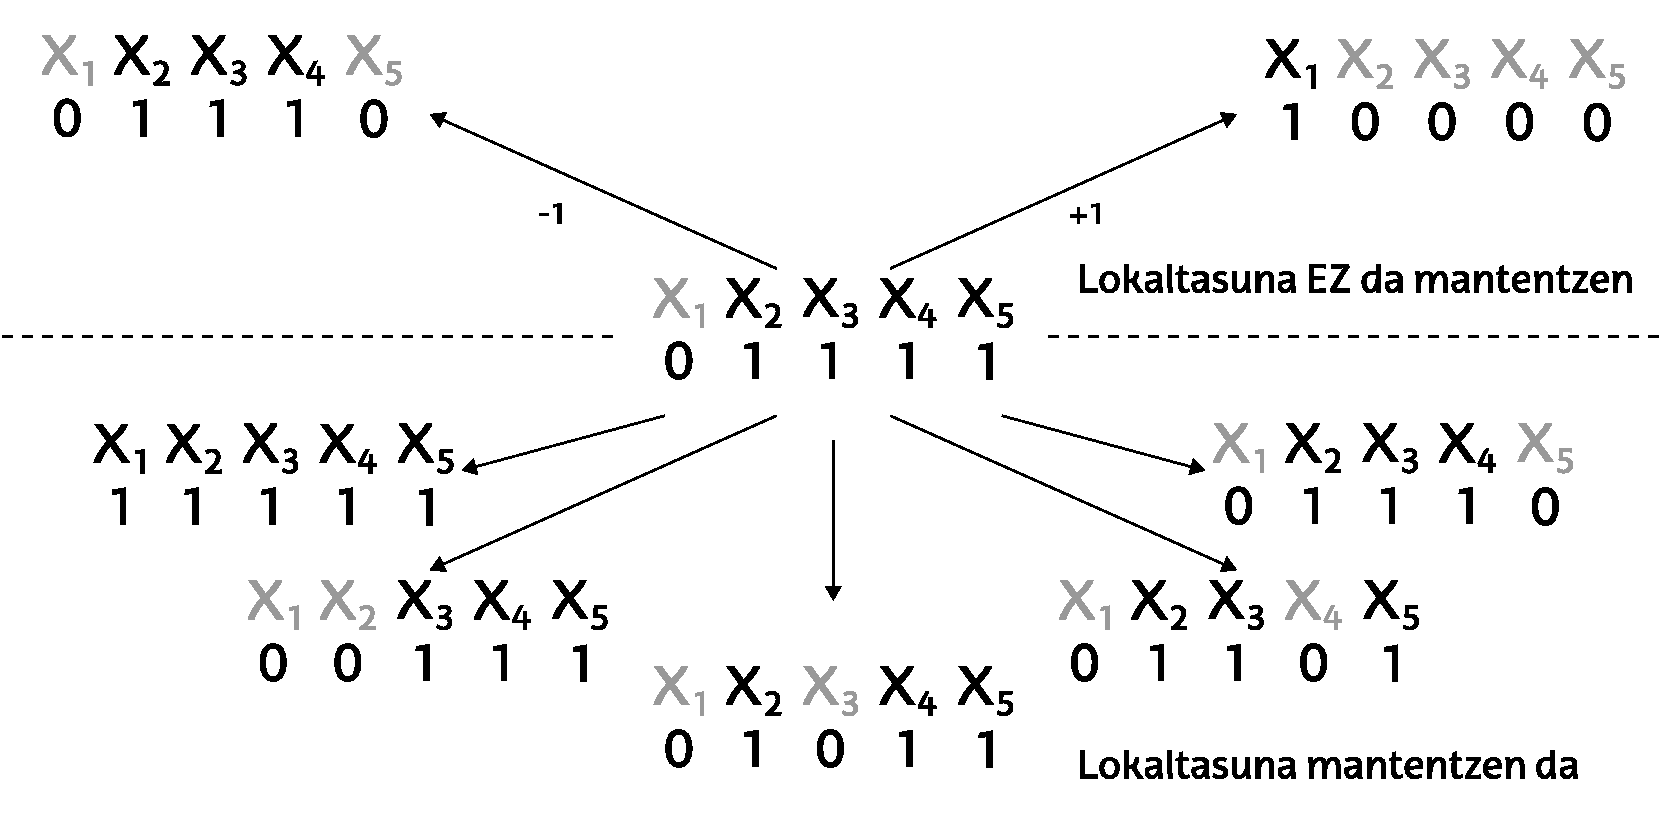
\includegraphics [width=0.75\textwidth]{./Irudiak/lokaltasuna}
\caption{Bi ingurune ezberdinen adibidea. Goikoan bektore bitarrei 1 gehitzen/kentzen diogu inguruneko soluzioak lortzeko. Eskuman dagoen soluzioan ikus daitekeen bezala, lokaltasuna ez da mantentzen, soluzioak elkarrengandik oso ezberdinak direlako. Beheko ingurunea \textit{flip} eragiketan oinarritzen da. Kasu honetan sortutako soluzio guztiak antzerakoak dira.}
\label{fig:locality}
\end{figure}

Soluzioak bektoreen bidez kodetzen direnean, inguruneak definitzeko \zkk distantzia\skk\ kontzeptua erabili ohi da, esplizituki zein inplizituki. Era honetan, bi soluzio bata bestearen ingurunean daudela esango dugu baldin eta beraien arteko distantzia finkaturiko kopuru bat baino txikiagoa bada. Edozein bi soluzio, $s$ eta $s^\prime$ arteko distantzia, $d(s,s^\prime)$ funtzioaz adierazten badugu, ingurunearen definizio orokorra ondorengoa izango da:

\begin{align}
N(s;k) = \{s^\prime\in {\cal S}\ |\ d(s,s^\prime)\leq k\}
\end{align}

Bektore motaren arabera distantzia ezberdinak erabil ditzakegu. Jarraian adibide hedatuenak ikusiko ditugu.
\paragraph{}
\noindent{\bf Bektore errealak} - Bektore errealekin dihardugunean euklidearra da gehien erabiltzen den distantzia

\begin{eqnarray*}
d_e(s,s^\prime) = \sqrt{\sum_{i=1}^n (s_i^\prime - s_i)^2}
\end{eqnarray*}

Ingurune tamainari erreparatuz, zenbaki errealekin dihardugunez, infinitu soluzio izango ditugu edozein soluzioren ingurunean. Euklidearra distantziarik ezagunena izan arren, badira beste metrika batzuk ere bektore errealen arteko distantzia neurtzeko -- Manhanttan- edo Chevyshev-distantziak, besteak beste --.
\paragraph{}
\noindent{\bf Bektore kategorikoak eta bitarrak} - Bektoreetan dauden aldagaiak kategorikoak direnean, bi bektoreen arteko distantzia neurtzeko metrikarik ezagunena Hamming-ek proposatutakoa da: $d_h(s,s^\prime) = \sum_{i=1}^n I[s_i\neq s_i^\prime ]$, non $I$ funtzioa adierazlea den, eta 1 balioa hartzen duen bere argumentua egia denean, eta 0 beste kasuan. Hortaz, Hamming-distantziak posizioz posizioko desberdintasunak neurtzen ditu. Hamming-distantzia inguruneak definitzeko erabiltzen denean, ohikoena 1 distantziara dauden soluzioetara mugatzea da, hau da:

\begin{align}\label{eq:hamming1_neigh}
N_{h}(s;1) = \{s^\prime\in {\cal S}\ |\ d_h(s,s^\prime) = 1\}
\end{align}

Algoritmoak diseinatzean oso garrantzitsua da ingurunearen tamaina aztertzea. Aurreko operadorea $n$ tamainako bektore bitar bati aplikatzen badiogu, $s$ soluzioaren bizilagun kopurua $|N(s)| = n$ izango da, posizio bakoitza aldatzeko aukera bakarra baitaukagu. Bektore kategorikoetan, posizio bakoitzean $r_i$ balio hartzeko aukera dagoenean, ingurunearen tamaina $|N(s)| = \sum_{i=1}^n (r_i - 1)$ izango da. 

Bestalde, ondoko ekuazioak, edozein distantziarako ingurune funtzio orokor bat adierazten du-- distantzia maximoa bektorearen tamaina dela kontutan hartuz, betiere  --.:

\begin{align}
N_{h}(s;k) = \{s^\prime\in {\cal S}\ |\ d_h(s,s^\prime) \leq k\}
\end{align}

Ikus dezagun adibide bat, \code{metaheuR} paketea erabiliz. Motxilaren problema erabiliko dugu eta, horretarako, lehenengo, ausazko problema bat eta soluzio bat sortuko ditugu. Pisua eta balioa korrelaturik egoteko, elementu bakoitzaren pisua lortzeko, haren balioari ausazko kopuru bat gehituko diogu. Gero, motxilaren kapazitatea definitzeko ausaz aukeratutako $\frac{n}{2}$ elementuen pisuak batuko ditugu. Azkenik, elementu bakoitza aukeratzeko probabilitatea heren batean ezarriz, ausazko soluzio bat sortuko dugu.

\begin{knitrout}
\definecolor{shadecolor}{rgb}{1, 1, 1}\color{fgcolor}\begin{kframe}
\begin{alltt}
\hlstd{> }\hlkwd{library}\hlstd{(metaheuR)}
\hlstd{> }\hlstd{n} \hlkwb{<-} \hlnum{10}
\hlstd{> }\hlstd{rnd.value} \hlkwb{<-} \hlkwd{runif}\hlstd{(n)} \hlopt{*} \hlnum{100}
\hlstd{> }\hlstd{rnd.weight} \hlkwb{<-} \hlstd{rnd.value} \hlopt{+} \hlkwd{runif}\hlstd{(n)} \hlopt{*} \hlnum{50}
\hlstd{> }\hlstd{max.weight} \hlkwb{<-} \hlkwd{sum}\hlstd{(}\hlkwd{sample}\hlstd{(rnd.weight,} \hlkwc{size}\hlstd{=n} \hlopt{/} \hlnum{2}\hlstd{,} \hlkwc{replace}\hlstd{=}\hlnum{FALSE}\hlstd{))}
\hlstd{> }\hlstd{knp} \hlkwb{<-} \hlkwd{knapsackProblem}\hlstd{(}\hlkwc{weight}\hlstd{=rnd.weight,} \hlkwc{value}\hlstd{=rnd.value,} \hlkwc{limit}\hlstd{=max.weight)}
\hlstd{> }\hlstd{rnd.sol} \hlkwb{<-} \hlkwd{runif}\hlstd{(n)} \hlopt{<} \hlnum{1} \hlopt{/} \hlnum{3}
\end{alltt}
\end{kframe}
\end{knitrout}

Kontutan hartu behar da motxilaren probleman soluzio guztiak --azpi-multzo guztiak, alegia-- ez direla bideragarriak. Eta beraz, ausazko soluzio bat sortzean, elementu edo objektu bat aukeratzeko probabilitatea handitzen badugu, soluzio bideraezinak lortzea probableagoa izango da. Edozein kasutan, sortutako soluzioa bideraezina izan daitekeenez, lehenengo pausua soluzioa zuzentzea izango da. Gero, \zkk flip\skk\ operadorea erabiliko dugu inguruneko soluzioak sortzeko. Operadore honek Hamming-en bat distantziara dauden soluzioak esleituko dizkio inguruneari. Nahiz eta uneko soluzioa bideragarria izan, ingurunekoak bideraezinak izan daitezke, beraz, pausu bakoitzean inguruneko soluzioa bideragarria den ala ez aztertu beharko dugu. 

\begin{knitrout}
\definecolor{shadecolor}{rgb}{1, 1, 1}\color{fgcolor}\begin{kframe}
\begin{alltt}
\hlstd{> }\hlstd{rnd.sol} \hlkwb{<-} \hlstd{knp}\hlopt{$}\hlkwd{correct}\hlstd{(rnd.sol)}
\hlstd{> }\hlkwd{which}\hlstd{(rnd.sol)}
\end{alltt}
\begin{verbatim}
## [1] 2 9
\end{verbatim}
\begin{alltt}
\hlstd{> }\hlstd{flip.ngh} \hlkwb{<-} \hlkwd{flipNeighborhood}\hlstd{(}\hlkwc{base}\hlstd{=rnd.sol,} \hlkwc{random}\hlstd{=}\hlnum{FALSE}\hlstd{)}
\hlstd{> }\hlkwa{while}\hlstd{(}\hlkwd{hasMoreNeighbors}\hlstd{(flip.ngh)) \{}
\hlstd{+ }  \hlstd{ngh} \hlkwb{<-} \hlkwd{nextNeighbor}\hlstd{(flip.ngh)}
\hlstd{+ }  \hlstd{is.valid} \hlkwb{<-} \hlkwd{ifelse}\hlstd{(}\hlkwc{test}\hlstd{=knp}\hlopt{$}\hlkwd{valid}\hlstd{(ngh),}
\hlstd{+ }                    \hlkwc{yes}\hlstd{=}\hlstr{"bideragarria"}\hlstd{,}
\hlstd{+ }                    \hlkwc{no}\hlstd{=}\hlstr{"bideraezina"}\hlstd{)}
\hlstd{+ }  \hlkwd{message}\hlstd{(}\hlstr{"Inguruneko soluzio "}\hlstd{, is.valid,} \hlstr{": "}\hlstd{,}
\hlstd{+ }          \hlkwd{paste}\hlstd{(}\hlkwd{which}\hlstd{(ngh),} \hlkwc{collapse}\hlstd{=}\hlstr{","}\hlstd{))}
\hlstd{+ }\hlstd{\}}
\end{alltt}


{\ttfamily\noindent\itshape\color{messagecolor}{\#\# Inguruneko soluzio bideragarria: 1,2,9\\\#\# Inguruneko soluzio bideragarria: 9\\\#\# Inguruneko soluzio bideragarria: 2,3,9\\\#\# Inguruneko soluzio bideragarria: 2,4,9\\\#\# Inguruneko soluzio bideragarria: 2,5,9\\\#\# Inguruneko soluzio bideragarria: 2,6,9\\\#\# Inguruneko soluzio bideragarria: 2,7,9\\\#\# Inguruneko soluzio bideragarria: 2,8,9\\\#\# Inguruneko soluzio bideragarria: 2\\\#\# Inguruneko soluzio bideragarria: 2,9,10}}\end{kframe}
\end{knitrout}

Goiko kodean ikus daitekeen bezala, \code{metaheuR} paketean inguruneak korritzeko bi funtzio aurki ditzakegu: \code{hasMoreNeighbors} eta \code{nextNeighbor}. Izenek adierazten duten bezala, lehenengo funtzioak ingurunean oraindik bisitatu gabeko soluzioren bat dagoen esaten digu eta, bigarrenak, bisitatu gabeko hurrengo soluzioa itzultzen du. Horrez gain, badago beste funtzio bat, \code{resetNeighborhood}, ingurune objektua berrabiarazteko. Informazio gehiago lor dezakezu R-ko terminalean \code{?resetNeighborhood} tekleatuz.

\paragraph{}
\noindent{\bf Permutazioak} - Permutazioen arteko distantziak neurtzeko metrikak existitu arren, ingurune operadore klasikoak ez dituzte zuzenean erabiltzen. Horren ordez, permutazioetan definitutako eragiketak erabili ohi dira, trukaketa eta txertaketa batik bat. 

Trukaketan -- \textit{swap} ingelesez --, permutazioaren bi posizio hartzen dira eta beraien balioak trukatzen dira. Adibidez, $21345$ permutazioaren 1. eta 3. posizioak trukatzen baditugu $31245$ permutazioa lortuko dugu. Formalki, trukaketa funtzioa, $t_r(s;i,j)$, defini dezakegu non $s^\prime = t_r(s;i,j)$ bada $s^\prime(i)=s(j)$, $s^\prime(j)=s(i)$ eta $\forall k\neq i,j$, $s^\prime(k)=s(k)$ beteko den. Funtzio honetan oinarriturik, ondoko ingurunea defini dezakegu:

\begin{align}
N_{2opt}(s) = \{t_r(s;i,j)|\ 1 \leq i,j\leq n,  \forall i > j\}
\end{align}

Ingurune honi \textit{2-opt} deritzo, bizilagun bakoitzea bi posizio bakarrik trukatzen baitira. Era berean, operadorea hedatu daiteke trukaketa gehiago eginez. Azkenik, hedatzeaz gain, operadorea murriztu ere egin ahal da, trukaketak elkarren ondoan dauden posizioetara soilik mugatuz. \textit{2-opt} ingurunearen trukaketa operadorea \code{ExchangeNeighborhood} klaseak inplementatzen du, eta ondoz-ondoko trukaketetara murriztutako bertsioa \code{SwapNeighborhood} klasearen bidez erabil daiteke.

Ingurunearen tamainari dagokionez, ondoz-ondoko posizioetan soilik trukaketak eginez $n-1$ ingurune soluzio izango ditugu; edozein bi posizio trukatzen baditugu, berriz, ingurunearen tamaina $n(n-1)$ izango da. Hau, jarraian dagoen adibidean ikus daiteke.

\begin{knitrout}
\definecolor{shadecolor}{rgb}{1, 1, 1}\color{fgcolor}\begin{kframe}
\begin{alltt}
\hlstd{> }\hlstd{n} \hlkwb{<-} \hlnum{10}
\hlstd{> }\hlstd{rnd.sol} \hlkwb{<-} \hlkwd{randomPermutation}\hlstd{(}\hlkwc{length}\hlstd{=n)}
\hlstd{> }
\hlstd{> }\hlstd{swp.ngh} \hlkwb{<-} \hlkwd{swapNeighborhood}\hlstd{(}\hlkwc{base}\hlstd{=rnd.sol)}
\hlstd{> }\hlstd{exchange.count} \hlkwb{<-} \hlnum{0}
\hlstd{> }\hlstd{swap.count} \hlkwb{<-} \hlnum{0}
\hlstd{> }\hlkwa{while}\hlstd{(}\hlkwd{hasMoreNeighbors}\hlstd{(swp.ngh)) \{}
\hlstd{+ }  \hlstd{swap.count} \hlkwb{<-} \hlstd{swap.count} \hlopt{+} \hlnum{1}
\hlstd{+ }  \hlkwd{nextNeighbor}\hlstd{(swp.ngh)}
\hlstd{+ }\hlstd{\}}
\hlstd{> }
\hlstd{> }\hlstd{ex.ngh} \hlkwb{<-} \hlkwd{exchangeNeighborhood}\hlstd{(}\hlkwc{base}\hlstd{=rnd.sol)}
\hlstd{> }\hlstd{exchange.count} \hlkwb{<-} \hlnum{0}
\hlstd{> }\hlkwa{while}\hlstd{(}\hlkwd{hasMoreNeighbors}\hlstd{(ex.ngh)) \{}
\hlstd{+ }  \hlstd{exchange.count} \hlkwb{<-} \hlstd{exchange.count} \hlopt{+} \hlnum{1}
\hlstd{+ }  \hlkwd{nextNeighbor}\hlstd{(ex.ngh)}
\hlstd{+ }\hlstd{\}}
\hlstd{> }
\hlstd{> }\hlstd{swap.count}
\end{alltt}
\begin{verbatim}
## [1] 9
\end{verbatim}
\begin{alltt}
\hlstd{> }\hlstd{exchange.count}
\end{alltt}
\begin{verbatim}
## [1] 45
\end{verbatim}
\end{kframe}
\end{knitrout}

Txertaketan -- \textit{insert} ingelesez --, elementu bat permutaziotik atera eta beste posizio batean sartzen dugu. Adibidez, $54123$ permutaziotik abiatuta, bigarren elementua laugarren posizioan txertatzen badugu, emaitza $51243$ izango da. Eragiketa $t_x(s;i,j)$ funtzioaren bidez adieraziko dugu -- $i$ elementua $j$ posizioan txertatu --, eta ingurunearen definizioa hauxe izango da:

\begin{align}
N_{in}(s) = \{t_x(s;i,j)|\ 1 \leq i,j\leq n, \forall i \neq j\}
\end{align}

Trukaketan bakarrik bi posiziotako balioak aldatzen dira; txertaketan, berriz, bi indizeen artean dauden posizio guztietako balioak aldatzen dira. Hori dela eta, ingurune operadore bakoitzaren erabilgarritasuna problemaren araberakoa izango da. Operadore hau ere \code{metaheuR} paketean aurki dezakegu, \code{InsertNeighborhood} klasean inplementaturik.

Bi ingurune operadore hauetaz gain, badiran literaturan beste zenbait operadore, inbertsio eragiketan oinarritutakoak esate baterako.


\subsection{Optimo lokalak}

Bilaketa lokalean -- oinarrizko bertsioan, behintzat -- soluzio batetik beste batera mugitzeko, uneko soluzioaren ingurunean, helburu funtzioaren balioa hobetzen duen bizilagun bat egon behar da\footnote{Helburu funtzioak soluzio jakin batean hartzen duen balioa, inglesezko {\it fitness} hitzarekin izendatzea ohikoa da. Horregatik, kapituluan zehar, bi adierazpideak erabiliko ditugu baliokide gisa.}. Inguruneko soluzio guztien fitness-a txarragoa baldin bada, orduan soluzio hau \textit{optimo lokala} dela esango dugu, eta bilaketa amaitu egingo da. Formalki, $s^*$ optimo lokala da baldin eta ondoko baldintza betetzen baldin badu:

\begin{align*}
\forall s \in N(s^*)\ \ f(s^*)\leq f(s)
\end{align*}

Aurreko ekuazioa {\cal S} osorako betetzen baldin bada, hau da, bilaketa espazio osorako, orduan, $s^*$ \textit{optimo globala} dela esango dugu.

\begin{figure}[t]
\centering
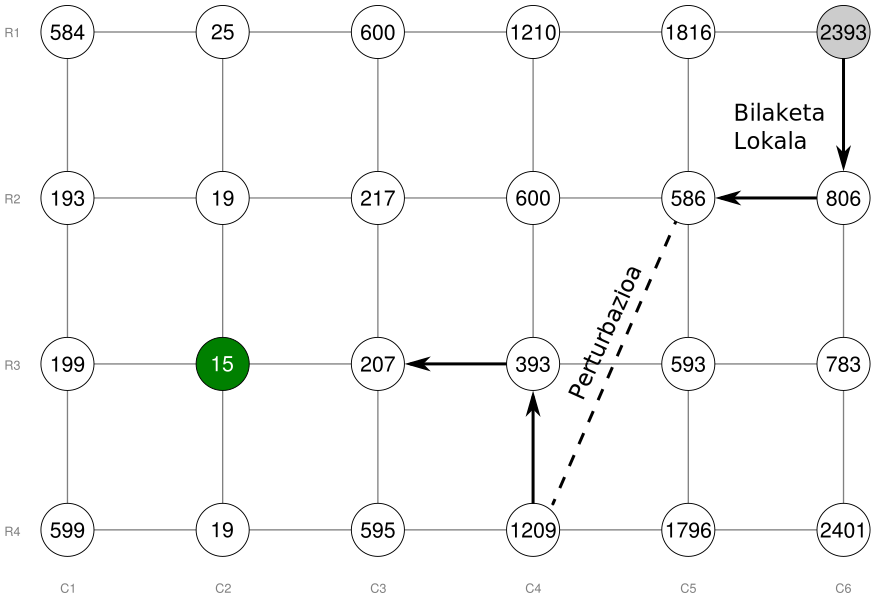
\includegraphics[width=0.66\linewidth]{./Irudiak/local_optimum}
\caption{Optimo lokalaren adibidea. Goiko eskumako soluziotik abiatzen bada bilaketa -- (R1,C6), grisean nabarmendua dagoen soluziotik, alegia --, eta pausu bakoitzean aukerarik onena aukeratzen badugu, geziek markatzen duten bidea jarraitu eta, bi pausutan, (R2,C5) soluzioan trabatuta geldituko gara. Soluzio hau optimo lokala da, bere inguruneko soluzio guztiak txarragoak baitira. Optimo lokalaren ebaluazioa 586 da, oso txarra optimo globalarekin alderatzen badugu --(R3,C2) soluzioa--.}
\label{fig:local_optimum}
\end{figure}

Definizio hauek kontutan hartuz, bilaketa lokala optimo lokal batean amaitzen dela beti ondorioztatzen dugu. Hauxe da, hain zuzen, bilaketa lokalaren ezaugarririk -- eta, aldi berean, desabantailarik -- nagusiena. Aintzat hartzekoa da optimo lokalak, nahiz eta bere inguruneko soluziorik onenak izan, nahiko soluzio txarrak izan daitezkeela, \ref{fig:local_optimum} irudian erakusten den bezala. Irudi honetan kapituluan zehar maiz erabiliko dugun grafiko mota bat ikus daiteke. Grafikoan, fikziozko problema baterako soluzio guztiak jasotzen dira, bakoitza borobil baten bidez adierazita; borobilen barruan soluzio bakoitzaren fitness-a dago idatzita. Ingurune funtzioa soluzioak lotzen dituzten marren bidez adierazten da; hala, bi soluzio lotuta badaude, bata bestearen ingurunean daudela diogu -- bizilagunak direla, alegia. 

\begin{tcolorbox}
\begin{ifexample}
\ref{fig:local_optimum} irudian agertzen diren geziek algoritmoak (R1,C6) soluziotik abiatuta egiten duen bidea erakusten dute. Pausu bakoitzean inguruneko soluziorik onena aukeratzen badugu, algoritmoa bi pausutan trabatuta geldituko da (R2,C5) soluzioan; soluzio honen fitness-a 586 da eta, bere ingurunean dauden soluzioen fitness-ak handiagoa direnez -- 1816, 806, 593 eta 600 --, ez dago helburu funtzioaren balioa hobetzen duen soluziorik. (R2,C5) optimo lokal bat da eta, optimo globalaren -- (R3,C2) -- fitness-a 15 dela kontutan hartuz, nahiko soluzio txarra ere bai.
\end{ifexample}
\end{tcolorbox}

Optimo lokaletatik ateratzeko hainbat estrategia planteatu dira literaturan, bilaketa lokalaren puntu batean edo bestean aldaketak proposatuz. Hauexek izango dira, hain justu, \ref{sec:BLHedapenak}. atalean aztergai izango ditugunak.

Ikusi dugunez, edozein soluziotik abiatuta, bilaketa lokala beti optimo lokal batean amaitzen da. Are gehiago, posible da bi soluzio ezberdinetatik hasita, bilaketa lokala soluzio berdinean amaitzea. Izan ere, optimo lokalek soluzioak \zkk erakartzen\skk\ dituzte, zulo beltzak balira bezala. Ideia hau \zkk erakarpen-arroa\skk\ -- \textit{basin of attraction}, ingelesez -- deritzon kontzeptuan formalizatzen da.

\begin{ifdefinition}{\bf erakarpen-arroa}
Izan bitez $N$ ingurune funtzioa, $f$ helburu funtzioa, $A(s;f,N): {\cal S}\rightarrow {\cal S}$ bilaketa lokaleko algoritmoa eta $s^*$ optimo lokala ($N$ ingurunerako eta $f$ funtziorako). $s^*$ optimo lokalaren erakarpen-arroa $\{s \in {\cal S} / A(s;N,f)=s^*\}$ soluzio multzoa da.
\end{ifdefinition} 

Erakarpen-arroa, definizioan ikus daitekeen legez, helburu funtzioaren, ingurunearen eta algoritmoaren araberakoa da. Alde batetik, ingurunearen eta helburu funtzioaren eragina begi bistakoa da. Bestetik, algoritmoak, ingurunea nola aztertzen den eta, bereziki, zein soluzio aukeratzen den ezartzen du; ondorioz, egiten dugun ibilbidean eragin handia izan dezake, \ref{fig:ls_selection_effect} irudian aukeraketa estrategiek duten eragina ilustratzen da.

\begin{figure}[t]
\centering
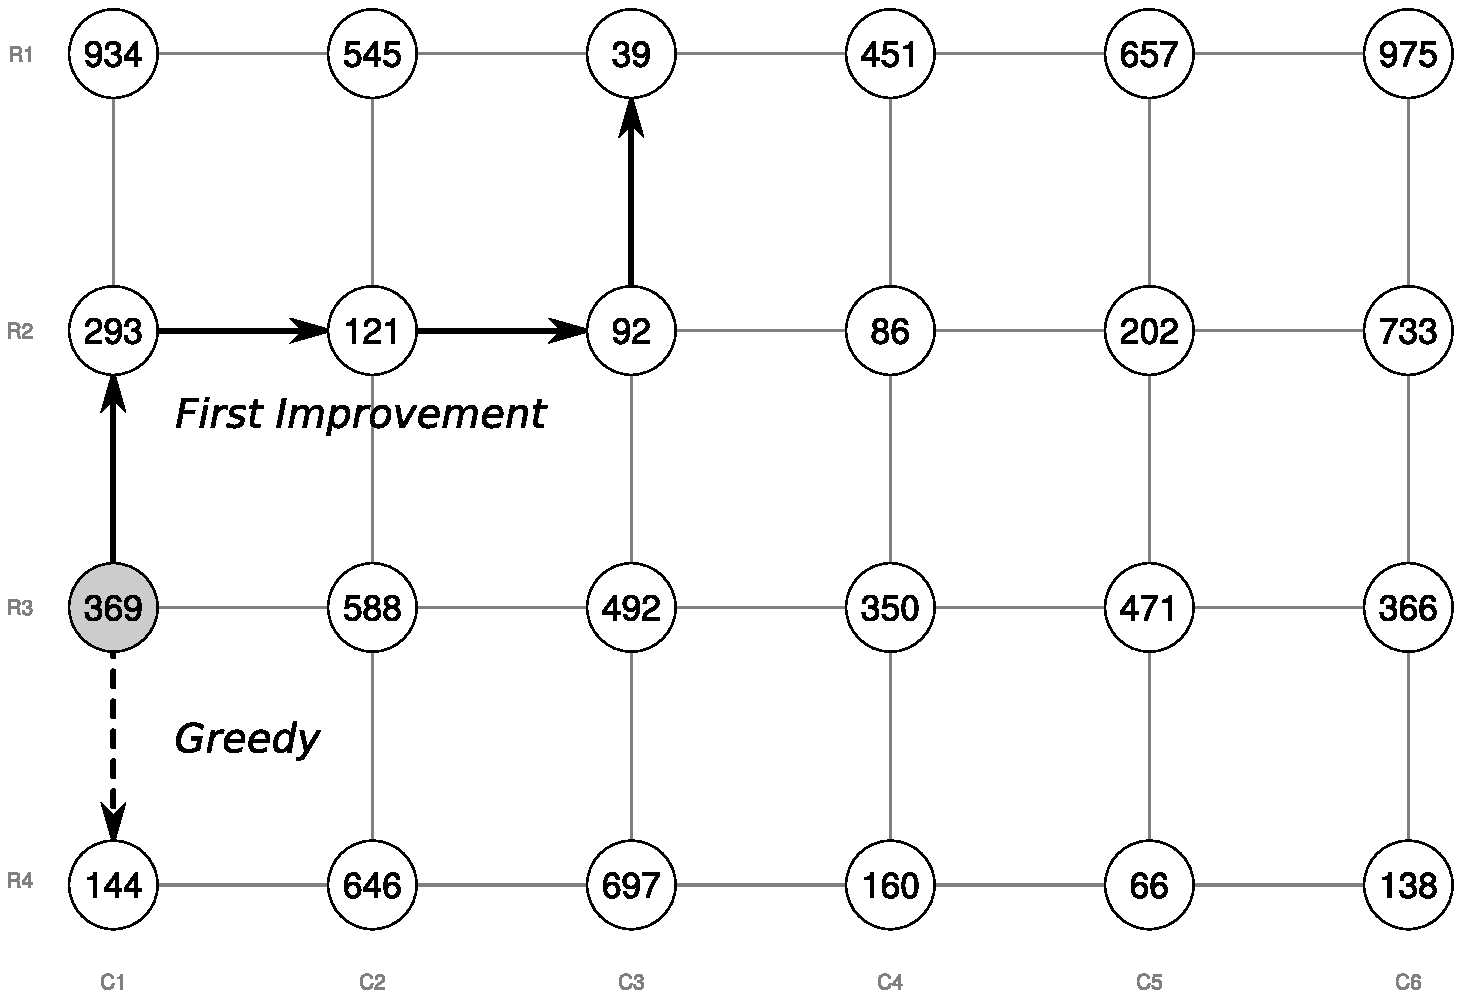
\includegraphics[width=0.66\linewidth]{./Irudiak/ls_selection_effect}
\caption{Inguruneko soluzioaren aukeraketaren efektua. Irudiak, soluzio berdinetik abiatuta -- (R3,C2), grisean nabarmendua -- bi estrategia ezberdin erabiliz egindako ibilbideak erakusten ditu. Lehenengo estrategia \textit{first improvement} motakoa da, hau da, helburu funtzioa hobetzen duen lehenengo soluzioa aukeratzen dugu -- inguruneko soluzioen ordena goikoa, eskumakoa, behekoa eta ezkerrekoa izanik --. Irizpide hau erabiliz egindako ibilbidea (R2,C1), (R2,C2), (R2,C3), (R1,C3) da, azken soluzio hau optimo lokala izanik. Bigarren estrategia gutiziatsua da -- \textit{greedy}-a, alegia --; aukeratzen dugun hurrengo soluzioa ingurunean dagoen onena izango da beti. Estrategia hau erabiliz pausu bakar batean (R4,C1) optimo lokalera ailegatzen gara.}
\label{fig:ls_selection_effect}
\end{figure}

\section{Bilaketa lokala}

Bilaketa lokalean oinarritutako edozein algoritmoren errendimendua, kodeketaren eta ingurunearen aukeraketaz gain, beste zenbait elementutan ere oinarritzen da. Lehenik eta behin, hasierako soluzioa nola aukeratzen dugun erabakitzea garrantzitsua da, aurreko atalean ikusi dugun moduan horren arabera optimo lokal batean edo bestean amaituko baita bilaketa. Bigarren oinarrizko elementua inguruneko soluzioen aukeraketa egiteko aplikatzen den estrategia da. Uneko soluzioaren ingurunean hainbat soluzio izango ditugu, baina, zein aukeratuko dugu hurrengo soluzioa izateko? Azkenik, gelditze irizpideak ere kontutan hartu beharreko faktoreak dira. Bilaketa lokala optimo lokal bat topatzen dugunean amaitzen da; dena dela, beste edozein algoritmotan bezala, denboran edota ebaluazio kopuruan oinarritutako gelditze irizpideak ere proposa ditzakegu\footnote{Informazio gehiago R-ren laguntzan duzu; \code{?basicLocalSearch} tekleatu laguntza zabaltzeko.}. \ref{alg:basicLS} algoritmoan oinarrizko bilaketa lokalaren sasikodea ikus daiteke.

\begin{ifalgorithm}[t]\label{alg:basicLS}
\begin{ifpseudo}{Oinarrizko bilaketa lokala}
\item \In\ $f$ helburu funtzioa, $s_0$ hasierako soluzioa, $N$ ingurune funtzioa
\item \Out\ $s^*$ soluzio optimoa
\item $s^*=s_0$
\item \Do
\item \T{$H=\{s^\prime \in N(s^*) | f(s^\prime)<f(s^*)\}$}
\item \T{\If $|H|>0$ }
\item \TT{Aukeratu $H$-n dagoen soluzio bat $s^\prime$ }
\item \TT{$s^* = s^\prime$}
\item \T{\EIf}
\item \While ($|H|>0$)
\end{ifpseudo}
\caption{Oinarrizko bilaketa lokalaren sasikodea. Uneko soluzioaren ingurunean fitness-a hobetzen duen soluzio bat bilatzen dugu. Horrelakorik badago, uneko soluzioa ordezkatzen dugu; ez badago, bilaketa amaitzen da.}
\end{ifalgorithm}

Sasikodean dagoen algorithmoa \code{metaheuR} paketeko \code{basicLocalSearch} funtzioak inplementatzen du. Funtzio honek zenbait parametro ditu, batzuk algoritmoarekin zerikusia dutenak eta beste batzuk problemari eta exekuzioari lotuta daudenak. Paketean dauden metaheuristika guztiek antzerako egitura izango dutenez, pausuz pausu aztertuko ditugu parametro hauek. Gauzak honela, parametroak hiru motakoak dira:
\begin{itemize}
\item Problemari lotutako parametroak - Bilaketa gidatzeko helburu funtzio bat behar dugu. Funtzio hau \code{evaluate} parametroaren bidez pasatuko diogu algoritmoari. Algoritmoen inplementazioa orokorra denez, gerta daiteke problema batzuetarako bideraezinak diren soluzioak agertzea. Problema mota hauekin lan egin ahal izateko, \code{metaheuR} paketeak soluzioen bideragarritasuna aztertu eta soluzio bideraezinak konpontzeko funtzioak parametro gisa sartzea ahalbidetzen du. Funtzio hauek problema bakoitzeko ezberdinak izango dira eta algoritmoari \code{valid} eta \code{correct} parametroen bidez pasatuko dizkiogu, hurrenez hurren.

\item Exekuzio kontrola - Badaude exekuzioaren zenbait aspektu kontrola ditzakegunak. Lehenik eta behin, algoritmoari baliabide konputazionalak mugatu diezazkiokegu, denbora, soluzio berrien ebaluazio kopurua edota iterazio kopurua finkatuz. Hau \code{cResource} objektuen  \code{cResource} parametroaren bidez kontrola dezakegu, bertan algoritmoak eskuragarri dituen baliabideak definituz. Horrez gain, \code{basicLocalSearch} funtzioak, algoritmoak gauzatzen duen bilaketaren progresioa bistaratzeko aukera ematen digu \code{verbose} parametroaren bidez. Era berean, progresioa taula batean gorde dezakegu, \code{do.log} parametroaren bidez.

\item Bilaketaren parametroak - Bilaketa lokala aplikatzeko hiru gauza behar ditugu, hasierako soluzioa, ingurune definizio bat eta inguruneko soluzio bat aukeratzeko prozedura. Hiru elementu hauek \code{initial.solution}, \code{neighborhood} eta \code{selector} parametroen bidez ezarri beharko ditugu. Horez gain, soluzio bideraezinak daudenean, hiru aukera ditugu, bideraezin diren soluzioak onartu, deskartatu edo konpontzea. Zein aukera erabili \code{non.valid} parametroaren bidez adiraziko dugu.
\end{itemize}

Jarraian \code{basicLocalSearch} funtzioaren eta bere parametro guztien erabilera adibide baten bidez aztertuko dugu. Adibiderako grafoen koloreztetze-problema bat sortuko dugu \code{graphColoringProblem} funtzioa erabiliz eta ausazko grafo bat hautatuz. Honela, \code{gcp} objektuak problemaren ebaluazio funtzioa eta soluzio bideragarriekin tratatzeko funtzioak gordeko ditu.

\begin{knitrout}
\definecolor{shadecolor}{rgb}{1, 1, 1}\color{fgcolor}\begin{kframe}
\begin{alltt}
\hlstd{> }\hlkwd{library}\hlstd{(igraph)}
\hlstd{> }\hlstd{n} \hlkwb{<-} \hlnum{25}
\hlstd{> }\hlstd{rnd.graph} \hlkwb{<-} \hlkwd{random.graph.game}\hlstd{(}\hlkwc{n}\hlstd{=n,} \hlkwc{p.or.m}\hlstd{=}\hlnum{0.25}\hlstd{)}
\hlstd{> }\hlstd{gcp} \hlkwb{<-} \hlkwd{graphColoringProblem} \hlstd{(}\hlkwc{graph}\hlstd{=rnd.graph)}
\end{alltt}
\end{kframe}
\end{knitrout}

Orain, algoritmoari emango dizkiogun baliabideak mugatuko ditugu. Gehienez, algoritmoak 10 segundu, helburu funtzioaren $100n^2$ ebaluazio edo algoritmoaren $100n$ iterazio erabili ahalko ditu.

\begin{knitrout}
\definecolor{shadecolor}{rgb}{1, 1, 1}\color{fgcolor}\begin{kframe}
\begin{alltt}
\hlstd{> }\hlstd{resources} \hlkwb{<-} \hlkwd{cResource}\hlstd{(}\hlkwc{time}\hlstd{=}\hlnum{10}\hlstd{,} \hlkwc{evaluations}\hlstd{=}\hlnum{100} \hlopt{*} \hlstd{n}\hlopt{^}\hlnum{2}\hlstd{,} \hlkwc{iterations}\hlstd{=}\hlnum{100} \hlopt{*} \hlstd{n)}
\end{alltt}
\end{kframe}
\end{knitrout}


Azkenik, bilaketarekin loturiko parametroei dagokienez, hasierako soluzio gisa soluzio tribiala sortuko dugu, non nodo bakoitzak kolore bat duen. Horrez gain, Hamming distantzian oinarritutako ingurune objektua sortuko dugu. Objetu honek ingurunea aztertu eta harekin lan egiteko beharrezko funtzioak gordeko ditu.

\begin{knitrout}
\definecolor{shadecolor}{rgb}{1, 1, 1}\color{fgcolor}\begin{kframe}
\begin{alltt}
\hlstd{> }\hlstd{colors} \hlkwb{<-} \hlkwd{paste}\hlstd{(}\hlstr{"C"}\hlstd{,} \hlnum{1}\hlopt{:}\hlstd{n,} \hlkwc{sep}\hlstd{=}\hlstr{""}\hlstd{)}
\hlstd{> }\hlstd{initial.solution} \hlkwb{<-} \hlkwd{factor} \hlstd{(colors,} \hlkwc{levels}\hlstd{=colors)}
\hlstd{> }\hlstd{h.ngh} \hlkwb{<-} \hlkwd{hammingNeighborhood}\hlstd{(}\hlkwc{base}\hlstd{=initial.solution)}
\end{alltt}
\end{kframe}
\end{knitrout}


Dena prest daukagu bilaketa abiaratzeko ...

\begin{knitrout}
\definecolor{shadecolor}{rgb}{1, 1, 1}\color{fgcolor}\begin{kframe}
\begin{alltt}
\hlstd{> }\hlstd{args} \hlkwb{<-} \hlkwd{list}\hlstd{()}
\hlstd{> }\hlstd{args}\hlopt{$}\hlstd{evaluate}         \hlkwb{<-} \hlstd{gcp}\hlopt{$}\hlstd{evaluate}
\hlstd{> }\hlstd{args}\hlopt{$}\hlstd{valid}            \hlkwb{<-} \hlstd{gcp}\hlopt{$}\hlstd{valid}
\hlstd{> }\hlstd{args}\hlopt{$}\hlstd{correct}          \hlkwb{<-} \hlstd{gcp}\hlopt{$}\hlstd{correct}
\hlstd{> }\hlstd{args}\hlopt{$}\hlstd{initial.solution} \hlkwb{<-} \hlstd{initial.solution}
\hlstd{> }\hlstd{args}\hlopt{$}\hlstd{neighborhood}     \hlkwb{<-} \hlstd{h.ngh}
\hlstd{> }\hlstd{args}\hlopt{$}\hlstd{selector}         \hlkwb{<-} \hlstd{firstImprovementSelector}
\hlstd{> }\hlstd{args}\hlopt{$}\hlstd{non.valid}        \hlkwb{<-} \hlstr{"correct"}
\hlstd{> }\hlstd{args}\hlopt{$}\hlstd{resources}        \hlkwb{<-} \hlstd{resources}
\hlstd{> }
\hlstd{> }\hlstd{bls} \hlkwb{<-} \hlkwd{do.call}\hlstd{(basicLocalSearch, args)}
\end{alltt}


{\ttfamily\noindent\itshape\color{messagecolor}{\#\# Running iteration 1. Best solution: 25\\\#\# Running iteration 2. Best solution: 24\\\#\# Running iteration 3. Best solution: 23\\\#\# Running iteration 4. Best solution: 22\\\#\# Running iteration 5. Best solution: 21\\\#\# Running iteration 6. Best solution: 20\\\#\# Running iteration 7. Best solution: 19\\\#\# Running iteration 8. Best solution: 18\\\#\# Running iteration 9. Best solution: 17\\\#\# Running iteration 10. Best solution: 16\\\#\# Running iteration 11. Best solution: 15\\\#\# Running iteration 12. Best solution: 14\\\#\# Running iteration 13. Best solution: 13\\\#\# Running iteration 14. Best solution: 12\\\#\# Running iteration 15. Best solution: 11\\\#\# Running iteration 16. Best solution: 10\\\#\# Running iteration 17. Best solution: 9\\\#\# Running iteration 18. Best solution: 8\\\#\# Running iteration 19. Best solution: 7\\\#\# Running iteration 20. Best solution: 6}}\begin{alltt}
\hlstd{> }\hlstd{bls}
\end{alltt}


{\ttfamily\noindent\itshape\color{messagecolor}{\#\# RESULTS OF THE SEARCH\\\#\# \\\#\# Best solution's evaluation: 6\\\#\# \\\#\# Algorithm: Basic Local Search\\\#\# \\\#\# Resource consumption:\\\#\# \\\#\# 	Time: 3.22650289535522\\\#\# \\\#\# 	Evaluations: 6339\\\#\# \\\#\# 	Iterations: 19\\\#\# \\\#\# None of the resources completely consumed\\\#\# \\\#\# \\\#\# You can use functions 'getSolution', 'getParameters' and 'getProgress' to get the list of optimal solutions, the list of parameters of the search and the log of the process, respectively}}\begin{alltt}
\hlstd{> }\hlstd{final.solution} \hlkwb{<-} \hlkwd{getSolution}\hlstd{(bls)}
\hlstd{> }\hlkwd{as.character}\hlstd{(final.solution)}
\end{alltt}
\begin{verbatim}
##  [1] "C2"  "C2"  "C4"  "C4"  "C2"  "C4"  "C8"  "C8"  "C2"  "C4"  "C2" 
## [12] "C2"  "C14" "C14" "C4"  "C14" "C4"  "C14" "C8"  "C21" "C21" "C21"
## [23] "C21" "C25" "C25"
\end{verbatim}
\begin{alltt}
\hlstd{> }\hlstd{plot.gpc.solution} \hlkwb{<-} \hlstd{gcp}\hlopt{$}\hlstd{plot}
\hlstd{> }\hlkwd{plot.gpc.solution}\hlstd{(}\hlkwc{solution}\hlstd{=final.solution,} \hlkwc{node.size}\hlstd{=}\hlnum{15}\hlstd{,} \hlkwc{label.cex}\hlstd{=}\hlnum{0.8}\hlstd{)}
\end{alltt}
\end{kframe}
\end{knitrout}

Bilaketa lokalak --eta, oro har, beste gainontzeko algoritmoek-- objektu berezi bat itzultzen dute, \code{mHResult} klasekoa. Bertan dagoen informazioa funtzio sorta baten bitartez lor daiteke; este baterako, \code{optima} funtzioak lortutako soluzio optimoa(k) itzultzen du, zerrenda batean. Bilaketa lokalak soluzio bakarra itzultzen duenez, soluzio hori listaren 1. posizioan egongo da. Soluzioa grafikoki bistaratzeko \code{graphColoringProblem} funtzioak itzultzen duen \code{plot} funtzioa erabil daiteke. Gainera, bilaketaren progresioa ere bistara dezakegu, \code{plotProgress} funtzioa erabiliz. \ref{fig:bls_gcp} irudiak problemarako soluzioa eta bilaketaren progresioa jasotzen ditu.

\begin{knitrout}
\definecolor{shadecolor}{rgb}{1, 1, 1}\color{fgcolor}\begin{kframe}
\begin{alltt}
\hlstd{> }\hlkwd{plotProgress}\hlstd{(bls,} \hlkwc{size}\hlstd{=}\hlnum{1.1}\hlstd{)} \hlopt{+} \hlkwd{labs}\hlstd{(}\hlkwc{y}\hlstd{=}\hlstr{"Evaluation"}\hlstd{)}
\end{alltt}
\end{kframe}
\end{knitrout}

\begin{figure}[t]
\subfigure[Problemaren soluzioa]{
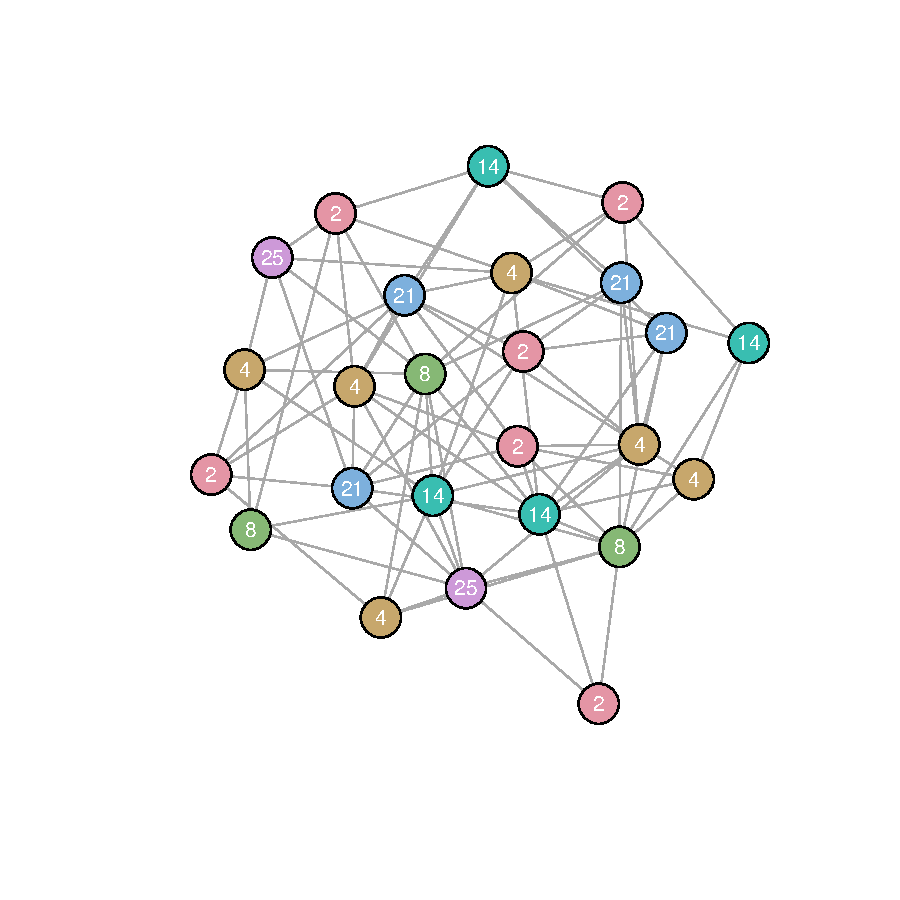
\includegraphics[width=0.39\textwidth] {./Irudiak/GC_4-1}
}\qquad
\subfigure[Bilaketaren progresioa]{
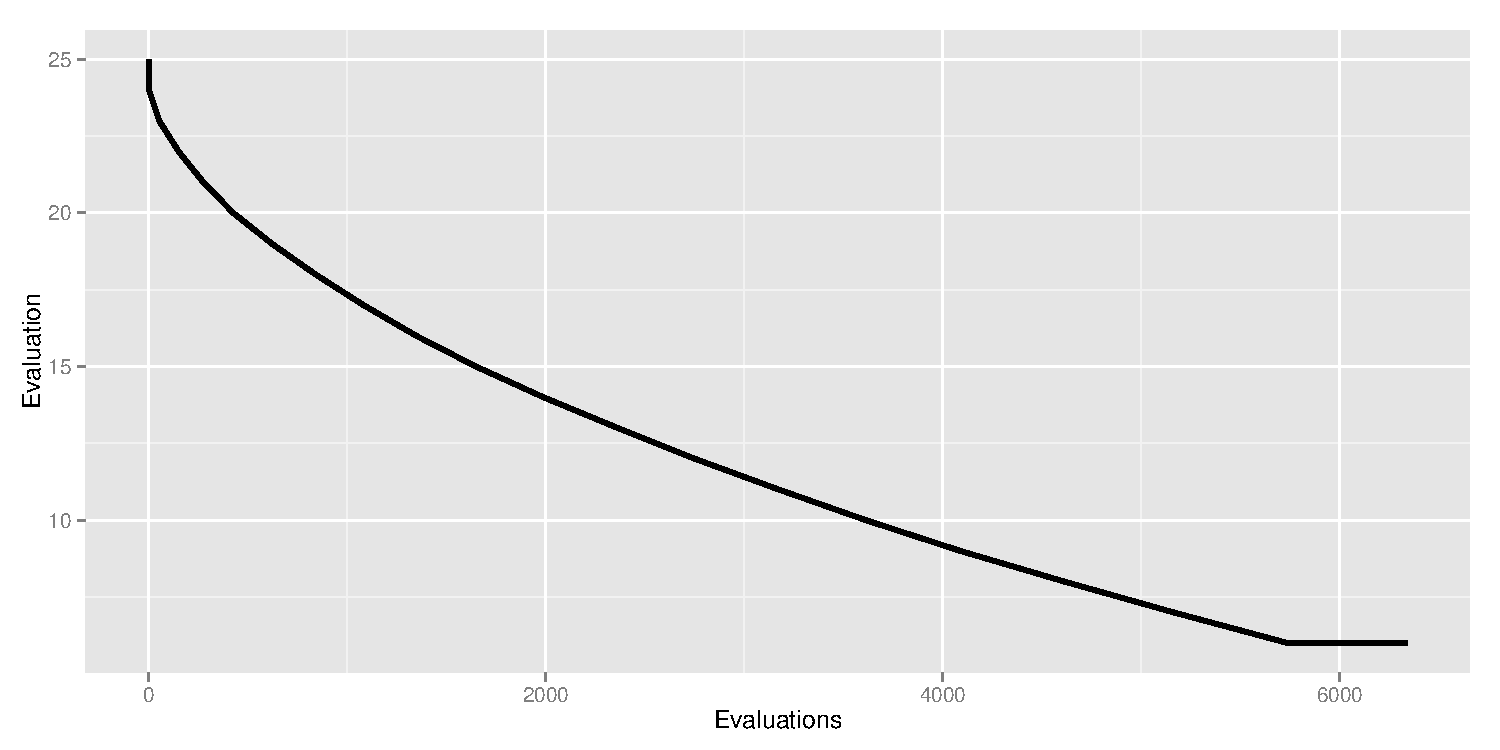
\includegraphics[width=0.59\textwidth] {./Irudiak/GC_5-1}
}\\
\caption{Grafoen koloreztatze-problemarako bilaketa lokalak topatutako soluzioa eta egindako bilaketaren progresioa. Bigarren grafiko honetan, X ardatzak ebaluazio kopurua adierazten du eta Y ardatzak uneko soluzioaren ebaluazioa --soluzioak erabiltzen dituen kolore kopurua, alegia--.}\label{fig:bls_gcp}
\end{figure}

Jarraian, bilaketa lokalean berebiziko garrantzia duten bi aspektu landuko ditugu: hasierako soluzioaren esleipena eta inguruneko soluzioaren aukeraketa.

\subsection{Hasierako soluzioaren aukeraketa}

Lehen aipatu bezala, bilaketa lokala soluzio batetik abiatuko da beti. Bilaketa nondik hasten den oso garrantzitsua da, horren arabera optimo lokal batean edo bestean amaituko baita bilaketa. Adibidez, hau argi ikusten da \ref{fig:local_optimum} irudian; (R1,C6) soluziotik hasten badugu bilaketa (C2,R5) soluzioan amaituko da. Gauza bera gertatzen da optimo lokaletik bertatik -- (C2,R5) --, goian dagoen soluziotik -- (C1,R5) -- edo bere eskuinean dagoen soluziotik -- (C2,R6) -- hasten bada prozesua. Beste edozein soluzio aukeratzen badugu, berriz, optimo globalera helduko gara. 

Hau ikusirik, bi dira bilaketa lokala hasieratzeko erabiltzen diren estrategia ohikoenak:

\begin{itemize}
\item \textbf{Ausazko soluzioak sortu} -  Ausaz aukeratzen da bilaketa espazioan dagoen soluzio bat eta hortik hasten da bilaketa. Metodo honen abantaila bere sinpletasuna da, ausazko soluzioak sortzea, kasu orokorrean, erraza izaten baita. Problemak murrizketa asko dituen kasuetan ordea, premisa honek ez du balio, baliozko ausazko soluzioak sortzea asko zaildu baitaiteke. Hala ere, estrategia honek alde txarrak ere baditu; alde batetik, hasierako soluzioa txarra bada, bilaketa prozesua luzea izan daiteke eta, bestetik, algoritmoa aplikatzen dugun bakoitzean emaitza, oro har, ezberdina izango da. 
\item \textbf{Soluzio onak eraiki} - Lehenengo kapituluan ikusi genuen problema bakoitza ebazteko metodo heuristiko espezifikoak diseina daitezkeela. Oro har, metodo hauek pausuz pausu eraikitzen dituzte soluzioak, urrats bakoitzean aukera guztietatik onena aukeratuz -- ingelesez metodo hauei \textit{constructive greedy} deritze, hau da algoritmo eraikitzaile gutiziatsuak edo jaleak --. Nahiko soluzio onak lortu arren, hauek ez dira zertan optimoak izan\footnote{Ez optimo globalak eta ezta lokalak ere.} eta, beraz, lortutako soluzioak bilaketa lokala hasieratzeko erabil daitezke. Estrategia hauek ausazko soluzioetatik abiatzeak baino emaitza hobeak lortzen ditu normalean, bilaketak iterazio gutxiago behar izaten baititu; konputazionalki ordea, garestiagoa da.
\end{itemize}

\subsection{Inguruneko soluzioaren aukeraketa}\label{sec:LS_selection}

Behin inguruneko soluzioen multzoa definiturik dugula, hurrengo pausua soluzio horien artean bat aukeratzeko irizpidea ezartzea da. Lehen aipatu bezala, bi dira, nagusiki, erabiltzen diren estrategiak. Lehenengo estrategian inguruneko soluzioak banan banan analizatzen dira eta fitness-a hobetzen duen lehenengo soluzioa aukeratzen da. Hurbilketan honetan, inguruneko soluzioen \zkk ordenazioa\skk\ oso garrantzitsua da, uneko soluzioa hobetzen duen lehenengo soluziora mugituko baikara. Bigarren estrategiak ingurune osoa arakatzen du eta fitness-a gehien hobetzen duen soluzioa aukeratzen du. Oro har, inguruneak txikiak direnean bigarren hurbilketa da interesgarriena baina, inguruneak handiak direnean, kostu konputazionala dela eta, bideraezina gerta daiteke estrategia hau.

\begin{tcolorbox}
\begin{ifexample}
Demagun problema baterako soluzioak bektore bitarren bidez kodetzen ditugula. Uneko soluzioa $(0,1,1,0,1)$ da dagokion fitness-a $25$ delarik. Ingurunea definitzeko \eqref{eq:hamming1_neigh} ekuazioan dagoen funtzioa erabiltzen badugu, inguruneko soluzioak hauexek izango dira:
\begin{itemize}
\item $s_1=(1,1,1,0,1)$; $f(s_1)=30$
\item $s_2=(0,0,1,0,1)$; $f(s_2)=24$
\item $s_3=(0,1,0,0,1)$; $f(s_3)=5$
\item $s_4=(0,1,1,1,1)$; $f(s_4)=27$
\item $s_5=(0,1,1,0,0)$; $f(s_5)=29$
\end{itemize} 
Inguruneko soluzioak lortzeko posizio bakoitzeko balioa banan-banan aldatu behar dugu. Lehenengo posiziotik abiatzen bagara, $s_2$ soluzioa izango da fitness-a hobetzen duen lehenengo soluzioa, bere ebaluazioa $24$ baita. Azken posiziotik abiatzen bagara, berriz, $s_3$ soluzioarekin geldituko ginateke, ebaluazioa $5$ baita. Kasu bakoitzean soluzio ezberdina aukeratu dugu lehenengo pausu honetan, hortaz, hurrengo urratsean izango dugun ingurunea ere ezberdina izango da. Hori dela eta, inguruneko soluzioen azterketa orden desberdinetan eginez, azken soluzioa ezberdina izan daiteke. Inguruneko soluziorik onena aukeratzen ordea, ordenak ez du garrantziarik eta beti soluzio berdina topatuko dugu, berdinketarik ez badago betiere.
\end{ifexample}
\end{tcolorbox}

Adibidean, soluzioen kodeketarekin zerikusia duen ordena erabiltzen da inguruneko soluzioak lortzeko. Horren ordez, esplorazioa ausaz ere egin daiteke.

Jarraian azaltzen den kodean ingurunearen azterketan ordenak duen eragina erakusten da. Lehenik eta behin, TSPlib repositorioan dagoen problema bat kargatuko dugu, \code{metaheuR} paketeko \code{tsplibParser} funtzioa erabiliz. TSPlib repositorioan TSP problemaren zenbait adibide ezberdin topa ditzakegu. Erabiliko dugun probleman Babariako 29 hiri izango ditugu. Hasierako soluzio gisa identitate permutazioa hartuko dugu.

\begin{knitrout}
\definecolor{shadecolor}{rgb}{1, 1, 1}\color{fgcolor}\begin{kframe}
\begin{alltt}
\hlstd{> }\hlstd{url} \hlkwb{<-} \hlkwd{system.file}\hlstd{(}\hlstr{"bays29.xml.zip"}\hlstd{,} \hlkwc{package} \hlstd{=} \hlstr{"metaheuR"}\hlstd{)}
\hlstd{> }\hlstd{cost.matrix} \hlkwb{<-} \hlkwd{tsplibParser}\hlstd{(url)}
\hlstd{> }\hlstd{n} \hlkwb{<-} \hlkwd{dim}\hlstd{(cost.matrix)[}\hlnum{1}\hlstd{]}
\hlstd{> }\hlstd{tsp.babaria} \hlkwb{<-} \hlkwd{tspProblem}\hlstd{(cost.matrix)}
\hlstd{> }\hlstd{csol} \hlkwb{<-} \hlkwd{identityPermutation}\hlstd{(n)}
\hlstd{> }\hlstd{csol}
\end{alltt}
\begin{verbatim}
## An object of class "Permutation"
## Slot "permutation":
##  [1]  1  2  3  4  5  6  7  8  9 10 11 12 13 14 15 16 17 18 19 20 21 22 23
## [24] 24 25 26 27 28 29
\end{verbatim}
\begin{alltt}
\hlstd{> }\hlstd{eval} \hlkwb{<-} \hlstd{tsp.babaria}\hlopt{$}\hlkwd{evaluate}\hlstd{(csol)}
\hlstd{> }\hlstd{eval}
\end{alltt}
\begin{verbatim}
## [1] 5752
\end{verbatim}
\end{kframe}
\end{knitrout}

Problema definitu ostean, hasierako soluzioaren ingurunea sortuko dugu. {\it 2-opt} ingurunea aukeratu dugu, ausazko eta ez-ausazko esplorazioak hautatuz. Lehenengoan inguruneko soluzioak ausazko orden batean aztertuko dira eta bigarrenean, ordea, kodeketaren araberako orden zehatz bat jarraituko da ingurunea arakatzeko.

\begin{knitrout}
\definecolor{shadecolor}{rgb}{1, 1, 1}\color{fgcolor}\begin{kframe}
\begin{alltt}
\hlstd{> }\hlstd{ex.nonrandom} \hlkwb{<-} \hlkwd{exchangeNeighborhood}\hlstd{(}\hlkwc{base}\hlstd{=csol,} \hlkwc{random}\hlstd{=}\hlnum{TRUE}\hlstd{)}
\hlstd{> }\hlstd{ex.random} \hlkwb{<-} \hlkwd{exchangeNeighborhood}\hlstd{(}\hlkwc{base}\hlstd{=csol,} \hlkwc{random}\hlstd{=}\hlnum{FALSE}\hlstd{)}
\end{alltt}
\end{kframe}
\end{knitrout}

Bilaketaren pausu bakoitzean inguruneko helburu funtzioa hobetzen duen lehenengo soluzioa aukeratzen badugu, hautatutako bi ordenazioak erabiliz emaitza ezberdinak lortuko ditugu. Ingurunea modu honetan arakatzeko, \code{firstImprovementSelector} funtzioa erabili dezakegu. Funtzio honek, uneko soluzioaren ingurunea arakatu du eta fitness-a hobetzen duen lehenengo soluzioa itzultzen du.

\begin{knitrout}
\definecolor{shadecolor}{rgb}{1, 1, 1}\color{fgcolor}\begin{kframe}
\begin{alltt}
\hlstd{> }\hlkwd{firstImprovementSelector}\hlstd{(}\hlkwc{neighborhood}\hlstd{=ex.nonrandom,} \hlkwc{evaluate}\hlstd{=tsp.babaria}\hlopt{$}\hlstd{evaluate,}
\hlstd{+ }                         \hlkwc{initial.solution}\hlstd{=csol,}\hlkwc{initial.evaluation}\hlstd{=eval)}\hlopt{$}\hlstd{evaluation}
\end{alltt}
\begin{verbatim}
## [1] 5684
\end{verbatim}
\begin{alltt}
\hlstd{> }\hlkwd{firstImprovementSelector}\hlstd{(}\hlkwc{neighborhood}\hlstd{=ex.random,} \hlkwc{evaluate}\hlstd{=tsp.babaria}\hlopt{$}\hlstd{evaluate,}
\hlstd{+ }                         \hlkwc{initial.solution}\hlstd{=csol,} \hlkwc{initial.evaluation}\hlstd{=eval)}\hlopt{$}\hlstd{evaluation}
\end{alltt}
\begin{verbatim}
## [1] 5478
\end{verbatim}
\end{kframe}
\end{knitrout}

Inguruneko soluziorik onena aukeratzen badugu, hautatutako bi ordenazioak erabiliz emaitza bera lortuko dugu, kasu guztietan inguruneko soluzio guztiak aztertzen baitira. Ingurunea aztertzeko estrategia hau \code{greedySelector} funtzioak inplementatzen du.

\begin{knitrout}
\definecolor{shadecolor}{rgb}{1, 1, 1}\color{fgcolor}\begin{kframe}
\begin{alltt}
\hlstd{> }\hlkwd{greedySelector}\hlstd{(}\hlkwc{neighborhood}\hlstd{=ex.nonrandom,} \hlkwc{evaluate}\hlstd{=tsp.babaria}\hlopt{$}\hlstd{evaluate,}
\hlstd{+ }               \hlkwc{initial.solution}\hlstd{=csol,} \hlkwc{initial.evaluation}\hlstd{=eval)}\hlopt{$}\hlstd{evaluation}
\end{alltt}
\begin{verbatim}
## [1] 5034
\end{verbatim}
\begin{alltt}
\hlstd{> }\hlkwd{greedySelector}\hlstd{(}\hlkwc{neighborhood}\hlstd{=ex.random,} \hlkwc{evaluate}\hlstd{=tsp.babaria}\hlopt{$}\hlstd{evaluate,}
\hlstd{+ }               \hlkwc{initial.solution}\hlstd{=csol,} \hlkwc{initial.evaluation}\hlstd{=eval)}\hlopt{$}\hlstd{evaluation}
\end{alltt}
\begin{verbatim}
## [1] 5034
\end{verbatim}
\end{kframe}
\end{knitrout}

Inguruneak handiak direnean ordenak oso eragin handia izan dezake eta, hortaz, heuristikoak erabil daitezke esplorazioa egiteko. Adibide gisa, Fred Glover-ek TSP problemarako proposatutako \textit{ejection chains} \citep{pesch1997} aipa daitezke. Gainera, metodo heuristikoez gain, tamaina handiko inguruneak era eraginkorrean zehazki aztertzeko algoritmoak ere badaude; hauetako adibide bat \textit{dynasearch}\citep{congram2000} algoritmoa da.


\subsection{Bilaketa lokalaren elementuen eragina}\label{sec:LS_elements}

Ikusi dugun bezala, bilaketa lokal arrunt bat aplikatzeko hiru aspektu aztertu behar ditugu. Lehenengoa, hasierako soluzioaren aukeraketa, bigarrena, erabiliko dugun ingurunearen diseinua eta, azkena, inguruneko soluzioaren aukeraketa. Atal honetan aspektu hauen eragina aztertuko dugu adibide baten bidez. 

Zehazki, aurreko atalean aurkeztutako Babariako hirien problema erabiliko dugu. Problema honetarako bi hasierako soluzio erabiliko ditugu, bat ausazkoa eta bestea algoritmo eraikitzaileak itzultzen duena.

\begin{knitrout}
\definecolor{shadecolor}{rgb}{1, 1, 1}\color{fgcolor}\begin{kframe}
\begin{alltt}
\hlstd{> }\hlstd{rnd.sol} \hlkwb{<-} \hlkwd{randomPermutation}\hlstd{(n)}
\hlstd{> }\hlstd{greedy.sol} \hlkwb{<-} \hlkwd{tspGreedy}\hlstd{(}\hlkwc{cmatrix}\hlstd{=cost.matrix)}
\hlstd{> }\hlstd{tsp.babaria}\hlopt{$}\hlkwd{evaluate}\hlstd{(rnd.sol)}
\end{alltt}
\begin{verbatim}
## [1] 6360
\end{verbatim}
\begin{alltt}
\hlstd{> }\hlstd{tsp.babaria}\hlopt{$}\hlkwd{evaluate}\hlstd{(greedy.sol)}
\end{alltt}
\begin{verbatim}
## [1] 2307
\end{verbatim}
\end{kframe}
\end{knitrout}

Ikusi daitekeenez, algoritmo eraikitzaileak (\code{tspGreedy}) ematen duen soluzioa ausazkoa baino askoz ere hobea da. Bi soluzio hauek hasierako soluzio gisa hartuz, bilaketa lokala aplikatu ahal dugu, {\it swap} ingurunea erabiliz. Gainera, pausu bakoitzean, inguruneko soluziorik onena aukera dezakegu ({\it greedy}) edo, bestela, uneko soluzioaren fitness-a hobetzen duen lehenengo soluzioa hartu ({\it first improvement (fi)}). Honenbestez, lau bilaketa ezberdin exekutatuko ditugu.

\begin{knitrout}
\definecolor{shadecolor}{rgb}{1, 1, 1}\color{fgcolor}\begin{kframe}
\begin{alltt}
\hlstd{> }\hlstd{eval} \hlkwb{<-} \hlstd{tsp.babaria}\hlopt{$}\hlstd{evaluate}
\hlstd{> }\hlstd{swp.ngh.rnd} \hlkwb{<-} \hlkwd{swapNeighborhood}\hlstd{(}\hlkwc{base}\hlstd{=rnd.sol)}
\hlstd{> }\hlstd{swp.ngh.greedy} \hlkwb{<-} \hlkwd{swapNeighborhood}\hlstd{(}\hlkwc{base}\hlstd{=greedy.sol)}
\hlstd{> }
\hlstd{> }\hlstd{args} \hlkwb{<-} \hlkwd{list}\hlstd{()}
\hlstd{> }\hlstd{args}\hlopt{$}\hlstd{evaluate}         \hlkwb{<-} \hlstd{eval}
\hlstd{> }\hlstd{args}\hlopt{$}\hlstd{initial.solution} \hlkwb{<-} \hlstd{rnd.sol}
\hlstd{> }\hlstd{args}\hlopt{$}\hlstd{neighborhood}     \hlkwb{<-} \hlstd{swp.ngh.rnd}
\hlstd{> }\hlstd{args}\hlopt{$}\hlstd{selector}         \hlkwb{<-} \hlstd{greedySelector}
\hlstd{> }\hlstd{args}\hlopt{$}\hlstd{verbose}          \hlkwb{<-} \hlnum{FALSE}
\hlstd{> }
\hlstd{> }\hlstd{swap.greedy.rnd.sol} \hlkwb{<-} \hlkwd{do.call}\hlstd{(basicLocalSearch, args)}
\hlstd{> }
\hlstd{> }\hlstd{args}\hlopt{$}\hlstd{selector}   \hlkwb{<-} \hlstd{firstImprovementSelector}
\hlstd{> }\hlstd{swap.fi.rnd.sol} \hlkwb{<-} \hlkwd{do.call}\hlstd{(basicLocalSearch, args)}
\hlstd{> }
\hlstd{> }\hlstd{args}\hlopt{$}\hlstd{initial.solution} \hlkwb{<-} \hlstd{greedy.sol}
\hlstd{> }\hlstd{swap.fi.greedy.sol}    \hlkwb{<-} \hlkwd{do.call}\hlstd{(basicLocalSearch, args)}
\hlstd{> }
\hlstd{> }\hlstd{args}\hlopt{$}\hlstd{selector}          \hlkwb{<-} \hlstd{greedySelector}
\hlstd{> }\hlstd{swap.greedy.greedy.sol} \hlkwb{<-} \hlkwd{do.call}\hlstd{(basicLocalSearch, args)}
\end{alltt}
\end{kframe}
\end{knitrout}

Azter dezagun zer nolako hobekuntza lortu dugun bilaketa lokalarekin, ausazko soluziotik abiatzen garenean.

\begin{knitrout}
\definecolor{shadecolor}{rgb}{1, 1, 1}\color{fgcolor}\begin{kframe}
\begin{alltt}
\hlstd{> }\hlstd{tsp.babaria}\hlopt{$}\hlkwd{evaluate}\hlstd{(rnd.sol)} \hlopt{-} \hlkwd{getEvaluation}\hlstd{(swap.greedy.rnd.sol)}
\end{alltt}
\begin{verbatim}
## [1] 1936
\end{verbatim}
\begin{alltt}
\hlstd{> }\hlstd{tsp.babaria}\hlopt{$}\hlkwd{evaluate}\hlstd{(rnd.sol)} \hlopt{-} \hlkwd{getEvaluation}\hlstd{(swap.fi.rnd.sol)}
\end{alltt}
\begin{verbatim}
## [1] 1317
\end{verbatim}
\end{kframe}
\end{knitrout}

Ikusi daitekeenez bilaketa lokalaren bidez, topatutako soluzioa hasierakoa baino askoz ere hobea da. Are gehiago, bilaketa prozesuko pausu bakoitzean inguruneko soluziorik onena aukeratzen badugu, hobekuntza handiagoa da. Halere, kontutan hartu behar da ebaluazio kopurua ere handiagoa dela kasu honetan.

\begin{knitrout}
\definecolor{shadecolor}{rgb}{1, 1, 1}\color{fgcolor}\begin{kframe}
\begin{alltt}
\hlstd{> }\hlkwd{getConsumedEvaluations}\hlstd{(}\hlkwd{getResources}\hlstd{(swap.greedy.rnd.sol))}
\end{alltt}
\begin{verbatim}
## [1] 337
\end{verbatim}
\begin{alltt}
\hlstd{> }\hlkwd{getConsumedEvaluations}\hlstd{(}\hlkwd{getResources}\hlstd{(swap.fi.rnd.sol))}
\end{alltt}
\begin{verbatim}
## [1] 276
\end{verbatim}
\end{kframe}
\end{knitrout}

Algoritmo eraikitzailearekin lortutako hasierako soluzioa, ausazko soluzioa baina hobea dela ikusi dugu. Hala ere, soluzio horri bilaketa lokala aplikatuz, soluzio oraindik hobea lortuko dugu, nahiz eta kasu honetan hobekuntza hain handia ez izan. 

\begin{knitrout}
\definecolor{shadecolor}{rgb}{1, 1, 1}\color{fgcolor}\begin{kframe}
\begin{alltt}
\hlstd{> }\hlstd{tsp.babaria}\hlopt{$}\hlkwd{evaluate}\hlstd{(greedy.sol)} \hlopt{-} \hlkwd{getEvaluation}\hlstd{(swap.greedy.greedy.sol)}
\end{alltt}
\begin{verbatim}
## [1] 56
\end{verbatim}
\end{kframe}
\end{knitrout}

Inguruneko soluzio guztietatik onena hartzeak emaitza hobeak ematen ditu --ausazko soluziotik abiatzen garenean, behintzat--, bilaketa espazioa sakonago aztertzen delako. Bilaketa sakonagoa egiteko beste era bat, {\it swap} ingurunearen ordez {\it 2-opt} ingurunea erabiltzean datza. Izan ere, lehen ikusi dugun bezala, {\it 2-opt} ingurunea {\it swap} ingurunea baino askoz ere handiagoa da.

\begin{knitrout}
\definecolor{shadecolor}{rgb}{1, 1, 1}\color{fgcolor}\begin{kframe}
\begin{alltt}
\hlstd{> }\hlstd{ex.ngh.rnd} \hlkwb{<-} \hlkwd{exchangeNeighborhood} \hlstd{(}\hlkwc{base}\hlstd{=rnd.sol)}
\hlstd{> }
\hlstd{> }\hlstd{args} \hlkwb{<-} \hlkwd{list}\hlstd{()}
\hlstd{> }\hlstd{args}\hlopt{$}\hlstd{evaluate}         \hlkwb{<-} \hlstd{eval}
\hlstd{> }\hlstd{args}\hlopt{$}\hlstd{initial.solution} \hlkwb{<-} \hlstd{rnd.sol}
\hlstd{> }\hlstd{args}\hlopt{$}\hlstd{neighborhood}     \hlkwb{<-} \hlstd{ex.ngh.rnd}
\hlstd{> }\hlstd{args}\hlopt{$}\hlstd{selector}         \hlkwb{<-} \hlstd{greedySelector}
\hlstd{> }\hlstd{args}\hlopt{$}\hlstd{verbose}          \hlkwb{<-} \hlnum{FALSE}
\hlstd{> }
\hlstd{> }\hlstd{ex.greedy.rnd.sol} \hlkwb{<-} \hlkwd{do.call}\hlstd{(basicLocalSearch, args)}
\hlstd{> }
\hlstd{> }\hlstd{tsp.babaria}\hlopt{$}\hlkwd{evaluate}\hlstd{(rnd.sol)} \hlopt{-} \hlkwd{getEvaluation}\hlstd{(ex.greedy.rnd.sol)}
\end{alltt}
\begin{verbatim}
## [1] 3951
\end{verbatim}
\begin{alltt}
\hlstd{> }\hlkwd{getConsumedEvaluations}\hlstd{(}\hlkwd{getResources}\hlstd{(ex.greedy.rnd.sol))}
\end{alltt}
\begin{verbatim}
## [1] 11775
\end{verbatim}
\end{kframe}
\end{knitrout}

Ikus daitekeen bezala, hobekuntza handiagoa da baina, inguruneak handiagoak direnez, baita ebaluazio kopurua ere.


\section{Bilaketa lokalaren hedapenak}\label{sec:BLHedapenak}

Aurreko atalean ikusi dugun legez, bilaketa lokala soluzioak areagotzeko prozedura egokia izan arren, desabantaila handi bat du; optimo lokaletan trabatuta gelditzen da. Arazo hau saihesteko -- soluzioen dibertsifikazioa suspertzeko, alegia -- bilaketa lokalak dituen lau aspektu nagusietan aldaketak sar ditzakegu bilaketan zehar: hasierako soluzioan, ingurunearen definizioan, inguruneko soluzioen aukeraketan eta helburu funtzioaren definizioan. Hurrengo ataletan hauetako elementu  bakoitzean aldaketak egiten dituzten algoritmo batzuk aurkeztuko ditugu.


\subsection{Hasieraketa anizkoitza}\label{sec:multistart}
Bilaketa lokala aplikatzean, soluzio bakoitzetik abiatuz optimo lokal batera heltzen gara; soluzio ezberdinetatik abiatzen bagara, optimo lokal ezberdinetara heldu gaitezke. Ideia hau da, hain zuzen ere, hasieraketa-anizkoitzeko bilaketa lokalak -- {\it Multistart Local Search}, inglesez-- inplementatzen duen (\ref{alg:randomMultistartLS} sasikodean ikusi daiteke). Algoritmoan agertzen diren \textit{generate\_random\_solution} eta \textit{local\_search} funtzioetan dago prozeduraren mamia, beraiek karakterizatuko baitute algoritmoaren performantzia. Lehenengoak, bilaketa espazioaren esplorazioa burutzen du. Bigarrena, aldiz, bere izenak adierazten duen bezala, soluzioen areagotzeaz arduratzen da.

\begin{ifalgorithm}[t]
\begin{ifpseudo}{Hasieraketa-anizkoitzeko bilaketa lokal orokorra}
\item \In\ $f$ helburu funtzioa
\item \In\ \textit{random\_solution}, \textit{stop\_criterion} eta \textit{local\_search} funtzioak
\item \Out\ $s^*$ soluzioa optimoa
\item $s$=\textit{generate\_random\_solution}
\item \While{!\textit{stop\_criterion}}
\item \T{$s^\prime$ = \textit{random\_solution}}
\item \T{$s^{\prime\prime}$ = \textit{local\_search}($s^\prime$)}
\item \T{\If({$f(s^{\prime\prime})<f(s)$}) $s=s^{\prime\prime}$}
\item \Done
\end{ifpseudo}
\caption{Hasieraketa anizkoitza erabiltzen duen bilaketa lokalaren hedapenaren sasikode orokorra}\label{alg:randomMultistartLS}
\end{ifalgorithm}

Hasteko, ausazko soluzioak sortzeko hainbat aukera ditugu. Horietako bat, soluzioak uniformeki ausaz sortzea da, hots, iterazio bakoitzean probabilitate berdinarekin espazioko edozein soluzio aukeratuko dugu eta bilaketa lokala soluzio horretatik hasiko dugu. Uniformeki ausazko soluzioetatik abiatzea, gehienetan, aukera erraza da; alabaina, ez da oso estrategia adimentsua. Gainera, murrizketa askoko problemetan ausazko soluzio bideragarriak sortzea zaila izan daiteke. Bilaketa hasieratzeko soluzio \zkk onak\skk\ eraikitzeko prozedura bat izanez gero, bi arazo hauek saihestu ditzakegu. Hain juxtu, hauxe da hurrengo atalean ikusiko ditugun ILS eta GRASP algoritmoak egiten dutena. 

\subsubsection{Bilaketa Lokala Iteratua (ILS)}

Bilaketa lokala berrabiarazteko uniformeki ausazko soluzioak erabili beharrean, ILS -- \textit{Iterated Local Search}, ingelesez -- algoritmoak uneko optimo lokala hartuko du oinarritzat. Ideia oso sinplea da; optimo lokal batean trabaturik gelditzen garenean, uneko soluzioa \zkk perturbatu\skk\ eta bertatik bilaketarekin jarraituko dugu. Optimo lokal berri batera heltzen garenean, soluzio hau onartuko dugunetz erabaki behar dugu. \ref{alg:ILS} algoritmoan ILS-aren sasikode orokorra ikusi daiteke.

\begin{ifalgorithm}[t]
\begin{ifpseudo}{Bilaketa Lokala Iteratua (ILS)}
\item \In\ $f$ helburu funtzioa
\item \In\ \textit{accept}, \textit{perturb}, \textit{stop\_criterion} eta \textit{local\_search} funtzioak
\item \In\ $s_0$ hasierako soluzioa
\item \Out\ $s^*$ soluzioa
\item $s = $ \textit{local\_search}($s_0$)
\item $s^* = s$
\item \While{!\textit{stop\_criterion}}
\item \T{$s^\prime$ = \textit{perturb}($s$)}
\item \T{$s^{\prime\prime}$ = \textit{local\_search}($s^\prime$)}
\item \T{\If (\textit{accept}($s^{\prime\prime}$)) $s=s^{\prime\prime}$}
\item \T{\If{($f(s^{\prime\prime})<f(s^*)$)} $s^*=s^{\prime\prime}$}
\item \Done
\end{ifpseudo}
\caption{Bilaketa Lokala Iteratuaren (ILS) sasikodea}\label{alg:ILS}
\end{ifalgorithm}

Algoritmo hau zehazteko bi prozedura berri definitu behar ditugu:

\begin{itemize}
\item \textbf{Perturbazioa} - Hasteko, optimo lokal batean trabaturik geratzean, hau nola perturbatuko den erabaki behar da. Soluzio baten inguruneko soluzio guztiak antzekoak direnez, optimo lokaletatik edo zehazki haien erakarpen-arroetatik ateratzeko, aldaketa nabarmenak egin behar dira (5 irudian adibide bat proposatzen da). Uneko soluzioa (R2,C5) izanik, perturbazio txikiegia egingo bagenu -- (R1,C5) soluziora mugitzea, adibidez --, berriro optimo lokal berdinean amaituko litzateke bilaketa. Perturbazioa nahiko handia bada, uneko optimo lokalaren erakarpen-arrotik aterako gara eta, definizioz, beste optimo lokal batean trabaturik geldituko gara. Kontutan hartzekoa da ordea, perturbazio prozedurak itzulitako soluzioa erabat ausazkoa bada --hau da, perturbazioa oso handia bada --, ILS algoritmoa ausazko hasieraketa anizkoitzeko algoritmoa bilakatuko dela. Beraz, perturbazio tamainaren aukeraketak eragina izango du algoritmoaren portaeran.

Perturbazioa definitzean inguruneko soluzioak definitzeko erabiltzen diren operazio mota berberak edo beste batzuk erabil daitezke. Esate baterako, permutazioetan oinarritzen den problema batean \textit{2-opt} ingurune operadorea erabiltzen badugu, \textit{k-opt} operadorea erabil daiteke soluzioak perturbatzeko. Perturbazioa trukaketan oinarritu beharrean, txertaketa ere erabil dezakegu, $k$ elementu hartu eta ausazko posizioetan sartuz. 

Perturbazioaren tamaina aurrez finkatu daiteke eta bilaketan zehar aldatu barik mantendu ala, bestalde, estrategia dinamikoak erabil daitezke, non perturbazioaren maila bilaketaren zehar aldatzen den.

Gainera, soluzioak perturbatzeko prozedura aurreratuetan, bilaketaren \zkk historia\skk\ ere erabil daiteke, soluzioaren zein osagai perturbatu eta zein ez erabakitzeko. Estrategia hauek \zkk memoria\skk\ kontzeptua erabiltzen dute eta memoria mota ezberdinak soluzioak areagotzeko eta dibertsifikatzeko balio dezakete.

\item \textbf{Optimo lokalak onartzeko irizpideak} - Uneko optimo lokala perturbatu ondoren bilaketa lokala aplikatzen da, optimo (berri) bat sortuz. Hurrengo iterazioan, lortutako optimo berria edo berriro optimo zaharra perturbatuko dugun erabaki behar da. Bi muturreko hurbilketa plantea daitezke: beti optimo berria onartu edo soilik unekoa baino hobea denean onartu. Lehendabiziko estrategiak dibertsifikazioa suspertzen du; bigarrena, berriz, soluzioak areagotzeko egokia da. Ohikoena tarteko zerbait erabiltzea da, optimo zaharraren eta berriaren ebaluazioen arteko  diferentzia kontutan hartuz. Esate baterako, optimoak era probabilistikoan onar daitezke, Boltzmann-en distribuzioa erabiliz, gero \textit{simmulated annealing} algoritmoan ikusiko dugun bezala. 
\end{itemize}

\begin{figure}[t]
\centering
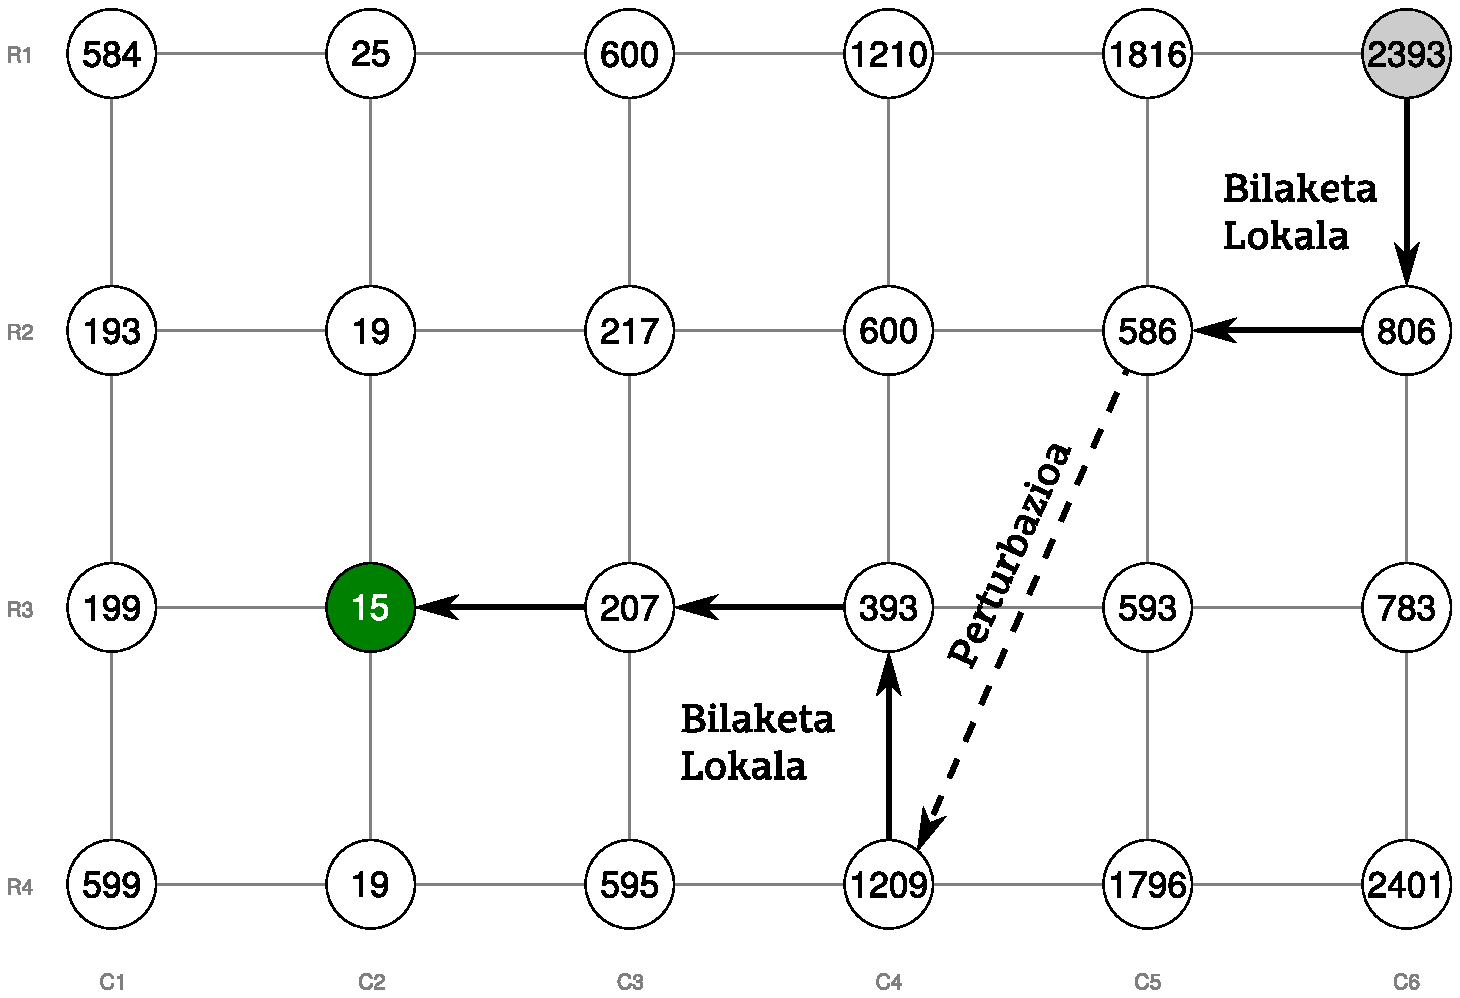
\includegraphics[width=0.66\linewidth]{./Irudiak/ILS}
\caption{ILS algoritmoaren funtzionamendua. Goiko eskumako soluziotik abiatzen bada bilaketa -- (R1,C6), grisean nabarmendua dagoen soluziotik, alegia --, (R2,C5) optimo lokalean trabatuta geldituko litzateke bilaketa lokala. Egoera desblokeatzeko soluzioa \zkk perturbatzen\skk\ dugu, (R3,C4) soluziora mugituz; hortik abiatuta bilaketa lokala aplikatzen dugu berriro, kasu honetan optimo globalera heldu arte}
\label{fig:ILS}
\end{figure}

\code{metaheuR} paketean, ILS-a \code{iteratedLocalSearch} funtzioan dago inplementatuta. Funtzio honen parametro gehienak \code{basicLocalSearch} funtzioaren berberak dira, inplementazioa funtzio horretan oinarritzen baita. Algoritmo honek ordea, hiru parametro berri izango ditugu:

\begin{itemize}
\item \code{perturb} - Parametro honen bidez soluzioak perturbatzeko erabiliko den funtzioa adieraziko diogu algoritmoari. \code{perturb} funtzioak parametro bakarra izango du, perturbatu behar den soluzioa, eta perturbazioa aplikatuz lortzen den soluzioa itzuliko du.
\item \code{accept} -  Parametro hau, soluzio berriak noiz onartzen ditugun definitzen duen funtzioa da. Gutxienez parametro bat izan beharko du, \code{delta}, soluzio berriaren eta zaharraren fitness balioen arteko diferentzia jasoko duena.
\item \code{num.restarts} - Optimo lokalak perturbatuz, bilaketa zenbat alditan berrabiarazi behar dugun esaten duen zenbaki osoa da.
\end{itemize}

Ikus dezagun adibide bat, TSPlib-eko problema bat erabiliz. Problema honetan Burma-ko 14 hirien arteko distantziak izango ditugu. Problema ebazteko ausazko soluzio batetik abiatuko dugu bilaketa. Ingurune gisa \textit{2-opt} erabiliko dugu (trukaketa orokorrak, ez bakarrik elkar-ondokoak) eta soluzioak perturbatzeko eragiketa bera erabiliko dugu baina behin baino gehiagotan aplikatuz; soluzio bati operazio hau ausaz aplikatzeko \code{shuffle} funtzioa erabil dezakegu.

\begin{knitrout}
\definecolor{shadecolor}{rgb}{1, 1, 1}\color{fgcolor}\begin{kframe}
\begin{alltt}
\hlstd{> }\hlstd{f} \hlkwb{<-} \hlkwd{paste}\hlstd{(}\hlstr{"http://www.iwr.uni-heidelberg.de/groups/comopt/software/TSPLIB95"}\hlstd{,}
\hlstd{+ }           \hlstr{"/XML-TSPLIB/instances/burma14.xml.zip"}\hlstd{,} \hlkwc{sep}\hlstd{=}\hlstr{""}\hlstd{)}
\hlstd{> }\hlstd{burma.mat} \hlkwb{<-} \hlkwd{tsplibParser}\hlstd{(f)}
\end{alltt}


{\ttfamily\noindent\itshape\color{messagecolor}{\#\# Processing file corresponding to instance burma14: 14-Staedte in Burma (Zaw Win)}}\begin{alltt}
\hlstd{> }\hlstd{n} \hlkwb{<-} \hlkwd{ncol}\hlstd{(burma.mat)}
\hlstd{> }\hlstd{burma.tsp} \hlkwb{<-} \hlkwd{tspProblem}\hlstd{(burma.mat)}
\hlstd{> }
\hlstd{> }\hlstd{init.sol} \hlkwb{<-} \hlkwd{randomPermutation}\hlstd{(n)}
\hlstd{> }\hlstd{ngh}      \hlkwb{<-} \hlkwd{exchangeNeighborhood}\hlstd{(init.sol)}
\hlstd{> }\hlstd{sel}      \hlkwb{<-} \hlstd{greedySelector}
\end{alltt}
\end{kframe}
\end{knitrout}

Segidan, optimo lokalak onartzeko irizpideak definituko ditugu. Kasu honetan, soluzioen arteko diferentzia 0 baina handiagoa izan beharko da, optimo lokal berria onartzeko. Hau da,  optimo lokal berria aurrekoa baina hobea izan behar da.

\begin{knitrout}
\definecolor{shadecolor}{rgb}{1, 1, 1}\color{fgcolor}\begin{kframe}
\begin{alltt}
\hlstd{> }\hlstd{th.accpet} \hlkwb{<-} \hlstd{thresholdAccept}
\hlstd{> }\hlstd{th} \hlkwb{<-} \hlnum{0}
\end{alltt}
\end{kframe}
\end{knitrout}

Perturbazio maila soluzioari aplikatuko dizkiogun trukaketa kopuruaren bidez kontrolatuko dugu. Beraz, trukaketa kopurua, gure perturbazio funtzioaren parametro bat izan beharko da\footnote{\code{iteratedLocalSearch} funtzioarekin (eta paketearen beste hainbat funtzioekin) arazorik ez izateko, pasatutako funtzioak \code{...} argumentua izan behar du gutxienez, nahiz eta gero barruan ez erabili.}.

\begin{knitrout}
\definecolor{shadecolor}{rgb}{1, 1, 1}\color{fgcolor}\begin{kframe}
\begin{alltt}
\hlstd{> }\hlkwd{set.seed}\hlstd{(}\hlnum{1}\hlstd{)}
\hlstd{> }\hlstd{perturbShuffle} \hlkwb{<-} \hlkwa{function}\hlstd{(}\hlkwc{solution}\hlstd{,} \hlkwc{ratio}\hlstd{,} \hlkwc{...}\hlstd{) \{}
\hlstd{+ }  \hlkwd{return}\hlstd{(}\hlkwd{shuffle}\hlstd{(}\hlkwc{permutation}\hlstd{=solution,} \hlkwc{ratio}\hlstd{=ratio))}
\hlstd{+ }\hlstd{\}}
\end{alltt}
\end{kframe}
\end{knitrout}

Honekin guztiarekin ILS algoritmoa exekutatu dezakegu perturbazio maila ezberdinekin:

\begin{knitrout}
\definecolor{shadecolor}{rgb}{1, 1, 1}\color{fgcolor}\begin{kframe}
\begin{alltt}
\hlstd{> }\hlstd{ratio} \hlkwb{<-} \hlnum{0.01}
\hlstd{> }
\hlstd{> }\hlstd{args} \hlkwb{<-} \hlkwd{list}\hlstd{()}
\hlstd{> }\hlstd{args}\hlopt{$}\hlstd{evaluate}         \hlkwb{<-} \hlstd{burma.tsp}\hlopt{$}\hlstd{evaluate}
\hlstd{> }\hlstd{args}\hlopt{$}\hlstd{initial.solution} \hlkwb{<-} \hlstd{init.sol}
\hlstd{> }\hlstd{args}\hlopt{$}\hlstd{neighborhood}     \hlkwb{<-} \hlstd{ngh}
\hlstd{> }\hlstd{args}\hlopt{$}\hlstd{selector}         \hlkwb{<-} \hlstd{sel}
\hlstd{> }\hlstd{args}\hlopt{$}\hlstd{perturb}          \hlkwb{<-} \hlstd{perturbShuffle}
\hlstd{> }\hlstd{args}\hlopt{$}\hlstd{ratio}            \hlkwb{<-} \hlstd{ratio}
\hlstd{> }\hlstd{args}\hlopt{$}\hlstd{accept}           \hlkwb{<-} \hlstd{th.accpet}
\hlstd{> }\hlstd{args}\hlopt{$}\hlstd{th}               \hlkwb{<-} \hlstd{th}
\hlstd{> }\hlstd{args}\hlopt{$}\hlstd{num.restarts}     \hlkwb{<-} \hlstd{r}
\hlstd{> }\hlstd{args}\hlopt{$}\hlstd{verbose}          \hlkwb{<-} \hlnum{FALSE}
\hlstd{> }
\hlstd{> }\hlstd{ils.1} \hlkwb{<-} \hlkwd{do.call}\hlstd{(iteratedLocalSearch, args)}
\hlstd{> }
\hlstd{> }\hlstd{args}\hlopt{$}\hlstd{ratio} \hlkwb{<-} \hlnum{0.25}
\hlstd{> }\hlstd{ils.25} \hlkwb{<-} \hlkwd{do.call}\hlstd{(iteratedLocalSearch, args)}
\hlstd{> }
\hlstd{> }\hlstd{args}\hlopt{$}\hlstd{ratio} \hlkwb{<-} \hlnum{1}
\hlstd{> }\hlstd{ils.100} \hlkwb{<-} \hlkwd{do.call}\hlstd{(iteratedLocalSearch, args)}
\hlstd{> }
\hlstd{> }\hlkwd{plotProgress}\hlstd{(}\hlkwc{result}\hlstd{=}\hlkwd{list}\hlstd{(}\hlkwc{ILS1}\hlstd{=ils.1,} \hlkwc{ILS25}\hlstd{=ils.25,} \hlkwc{ILS100}\hlstd{=ils.100))} \hlopt{+}
\hlstd{+ }  \hlkwd{facet_grid}\hlstd{(.} \hlopt{~} \hlstd{Group,} \hlkwc{scales}\hlstd{=}\hlstr{"free_x"}\hlstd{)} \hlopt{+} \hlkwd{labs}\hlstd{(}\hlkwc{y}\hlstd{=}\hlstr{"Evaluation"}\hlstd{)}
\end{alltt}
\end{kframe}
\end{knitrout}

\begin{figure}[t]
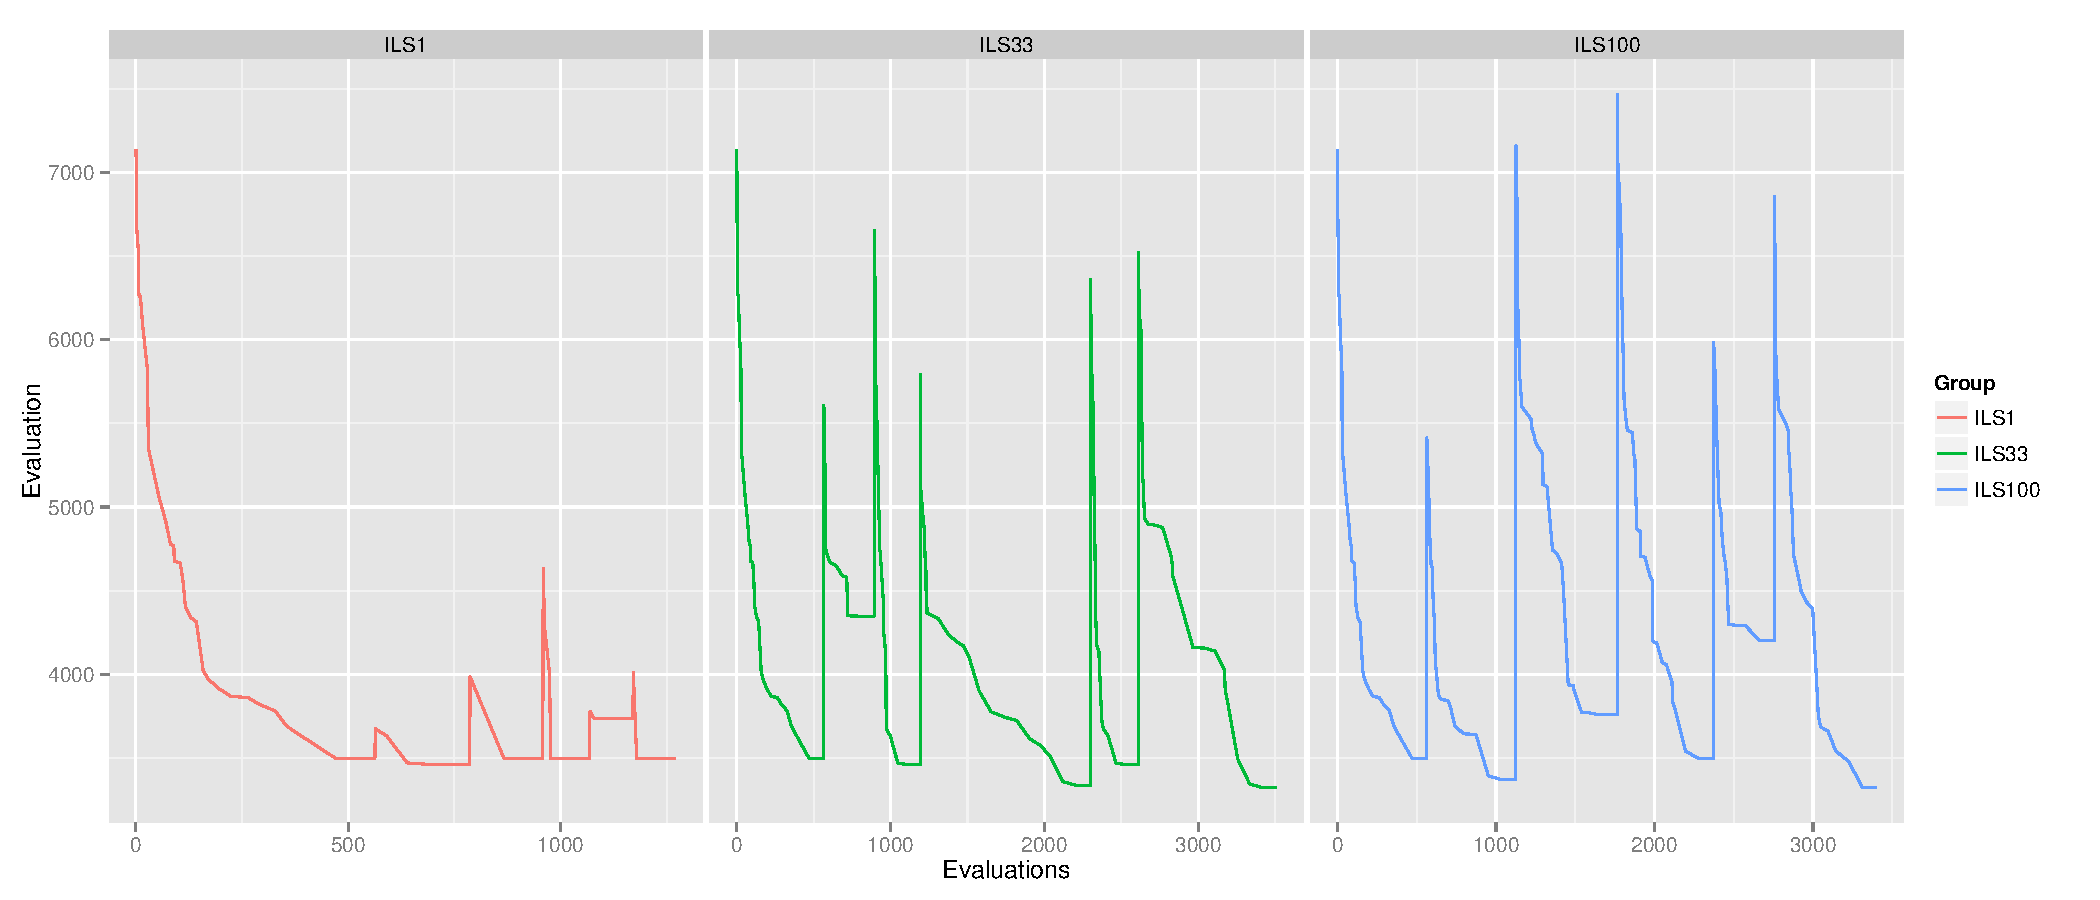
\includegraphics[width=\textwidth]{./Irudiak/Burma_2-1}
\caption{ILS algoritmoaren progresioa 14 hiriko TSP problema batean. Ezkerretik eskuinera, perturbazioaren ratioak 0.01, 0.25 eta 1 dira.}\ref{fig:ILS}
\end{figure}

Hiru bilaketa hauen progresioak \ref{fig:ILS} irudian ikus daitezke. Hirurak soluzio berdinetik hasten dira eta, pausu bakoitzean inguruko soluziorik onena aukeratzen dutenez, lehenengo jaitsiera berdina da hiru grafikoetan. Lehenengo optimo lokala topatzen den momentuan, ordea, diferentziak hasten dira. Ezkerretik eskuinera, lehenengo grafikoan soluzioak posizioen \%1 trukatuz perturbatzen dira; guztira soluzioak 14 posizio dituztenez, trukaketa bakar bat egiten da. Erdiko grafikoan perturbazioa \%25ekoa da, 3 trukaketa egiten dira, alegia. Azken grafikoan, berriz, 14 trukaketa egiten dira (posizioen \%100). Perturbazio txiki bat erabiltzen dugunean, lortutako soluzioaren ebaluazioa optimo lokalaren antzerakoa da (agertzen diren jauziak  ez dira oso altuak, alegia); geroz eta perturbazio handiagoa orduan eta diferentzia handiagoa soluzio berria eta optimoaren artean. Azken kasuan, perturbazioa oso handia da eta, beraz, optimo lokaletatik ateratzeko, soluzioak guztiz ausaz aukeratzen dira, hasieraketa anizkoitzeko algoritmoan bezala.


\subsubsection{GRASP algoritmoa}

Optimizazio problemak ebazteko ohikoa da metodo eraikitzaileak erabiltzea. Aurreko kapituluan ikusi genuen bezala, algoritmo hauek soluzioa pausuz pausu eraikitzen dute, urrats bakoitzean aukera guztietatik onena hautatuz. Era honetan, soluzio onak sortzen dira baina, hauek ez dute zertan optimoak izan, ez globalki eta ezta lokalki ere. Hori dela eta, behin soluzioa sortuta, bilaketa lokal bat erabil daiteke soluzioa areagotzeko. Alabaina, berdinketak egon ezean, metodo eraikitzaileek instantzia bakoitzeko soluzio bakarra eta beti berdina lortzen dute eta beraz hasieraketa bakarra ahalbidetzen dute.

Ideia hau apur bat landuz, metodo eraikitzaileak soluzio bakarra sortu beharrean soluzio multzo bat sortzeko egoki ditzakegu. Eta ondoren, \ref{alg:randomMultistartLS} algoritmoan agertzen den \textit{random\_solution} metodoak multzo horretatik ausazko soluzioak aterako ditu, bilaketa lokala hasieratzeko. Ideia hau GRASP \textit{Greedy Randomized Adaptative Search Procedure} algoritmoaren atzean dagoena da \cite{feo1989}.

Ausazko soluzio onak eraikitzeko, pausu bakoitzean aukerarik onena aukeratu beharrean \zkk hautagai zerrenda\skk\ bat izango dugu -- \textit{candidate list}, ingelesez --; algoritmoak zerrenda horretan dauden osagaiak ausaz aukeratuko ditu hasierako soluzioak eraikitzeko.

\begin{tcolorbox}
\begin{ifexample}
Demagun motxilaren problema ebatzi nahi dugula. Oso sinplea den algoritmo eraikitzaile bat ondorengoa da: lehenik eta behin, kalkulatu motxilan sartzen ditugun elementu bakoitzaren balioa/pisua ratioa eta gero, pausu bakoitzean, pisu-muga gaindiarazi ez duten elementuetatik, ratiorik handiena duena aukeratu. 

Algoritmo hau GRASP algoritmoaren ideiara modu errezean egokitu daiteke. Algoritmoaren iterazio bakoitzean hasierako soluzio bat eraikiko dugu pausu bakoitzean, ratiorik handiena duen elementua aukeratu beharrean ratio handiena duten $\%\alpha$ soluzioen artetik bat ausaz aukeratuz. Behin soluzioa eraikita, bilaketa lokala aplikatuko dugu lortutako soluzioa areagotzeko. 
\end{ifexample}
\end{tcolorbox}

Edozein problemari GRASP algoritmoa aplikatzeko, adibidean planteatzen den hasierako soluzio onak sortzeko estrategiaren antzerako prozedura bat diseinatu eta inplementatu beharko dugu. Funtzio honen parametro gehienak problema bakoitzarentzat ezberdinak izango dira baina, gainera, hautagaien zerrendaren luzeera $\alpha$ proportzio baten bidez adierazi beharko dugu. 

Adibide gisa, \code{metaheuR} paketean motxilaren problema GRASP algoritmoaren bitartez ebatzi ahal izateko, \code{graspKnapsack} funtzioa izango dugu. Funtzio honetan, hasteko, zenbait datu atera eta aldagai batzuk hasieratzen dira. Besteak beste, elementurik gabeko soluzio \zkk hutsa\skk sortuko dugu.





\begin{knitrout}
\definecolor{shadecolor}{rgb}{1, 1, 1}\color{fgcolor}\begin{kframe}
\begin{alltt}
graspKnapsack <- \hlkwd{function}(weight, value, limit, cl.size=0.25) \{
  size <- \hlkwd{length}(weight)
  ratio <- value / weight
  solution <- \hlkwd{rep}(FALSE, size)
  finished <- FALSE
\end{alltt}
\end{kframe}
\end{knitrout}

Soluzioa sortzeko, elementuak banan banan sartuko ditugu motxilan, eta honetarako, begizta bat izango dugu, motxila beteta ez dagoen bitartean errepikatuko dena. Begiztaren lehenengo pausuan, motxilan oraindik sartu gabeko elementuei atzematen diegu eta, uneko iterazioan, gure hautagai zerrendak izango duen tamaina kalkulatzen dugu (gogoratu hautagai zerrendaren tamaina urrats bakoitzean ditugun aukera kopuruaren proportzio bat bezala definitu dugula).

\begin{knitrout}
\definecolor{shadecolor}{rgb}{1, 1, 1}\color{fgcolor}\begin{kframe}
\begin{alltt}
  \hlkwd{while} (!finished) \{
    non.selected <- \hlkwd{which}(!solution)
    cl.n <- \hlkwd{max}(1, \hlkwd{round}(\hlkwd{length}(non.selected) * cl.size))
\end{alltt}
\end{kframe}
\end{knitrout}

Orain, ratioak ordenatu ondoren, lehenengo elementuak hartzen ditugu hautagai zerrenda gisa, eta horietatik bat ausaz aukeratzen dugu.

\begin{knitrout}
\definecolor{shadecolor}{rgb}{1, 1, 1}\color{fgcolor}\begin{kframe}
\begin{alltt}
    \hlstd{cl} \hlkwb{<-} \hlkwd{sort}\hlstd{(ratio[non.selected],} \hlkwc{decreasing}\hlstd{=}\hlnum{TRUE}\hlstd{)[}\hlnum{1}\hlopt{:}\hlstd{cl.n]}
    \hlstd{selected} \hlkwb{<-} \hlkwd{sample}\hlstd{(cl,} \hlnum{1}\hlstd{)}
\end{alltt}
\end{kframe}
\end{knitrout}

Bukatzeko, aukeratutako elementua soluzioan sartu eta aurrera jarraitzen da motxila betetzen ez den bitartean. Motxila bete egiten bada, sartutako azkeneko elementua atera eta begizta bukatu egingo da.

\begin{knitrout}
\definecolor{shadecolor}{rgb}{1, 1, 1}\color{fgcolor}\begin{kframe}
\begin{alltt}
    aux <- solution
    aux[ratio == selected] <- TRUE
    \hlkwd{if} (\hlkwd{sum}(weight[aux]) < limit) \{
      solution <- aux
    \}else\{
      finished <- TRUE
    \}
  \}
  \hlkwd{return}(solution)
\}
\end{alltt}
\end{kframe}
\end{knitrout}

Sortu dugun funtzioa, GRASP algoritmoa, guztiz ausazkoa den hasieraketa anizkoitzarekin alderatzeko erabil dezakegu, \code{cl.size} parametroarekin jolastuz. Lehenik eta behin, ausazko motxilaren problema bat sortuko dugu. Kasu honetan 50 elementu izango ditugu eta hauen balioa bi multzotan banatuko dugu. Elementu erdien balioak 0 eta 10 arteko ausazko zenbakiak izango dira; beste erdien balioak, 0 eta 25 tartetik ausaz hautatuko ditugu. Kasu guztietan pisua balioarekiko proportzionala izango da, faktorea ausazko zenbaki bat izanik. Limite gisa, ausaz aukeratutako 10 elementuen pisuaren batura erabiliko dugu.

\begin{knitrout}
\definecolor{shadecolor}{rgb}{1, 1, 1}\color{fgcolor}\begin{kframe}
\begin{alltt}
\hlstd{> }\hlstd{n} \hlkwb{<-} \hlnum{50}
\hlstd{> }\hlstd{values}  \hlkwb{<-} \hlkwd{c}\hlstd{(}\hlkwd{runif}\hlstd{(n} \hlopt{/} \hlnum{2}\hlstd{)} \hlopt{*} \hlnum{10}\hlstd{,}  \hlkwd{runif}\hlstd{(n} \hlopt{/} \hlnum{2}\hlstd{)} \hlopt{*} \hlnum{25}\hlstd{)}
\hlstd{> }\hlstd{weights} \hlkwb{<-} \hlstd{values} \hlopt{*} \hlkwd{rnorm}\hlstd{(n,} \hlnum{1}\hlstd{,} \hlnum{0.05}\hlstd{)}
\hlstd{> }\hlstd{limit}   \hlkwb{<-} \hlkwd{sum}\hlstd{(}\hlkwd{sample}\hlstd{(weights, n} \hlopt{/} \hlnum{5}\hlstd{))}
\end{alltt}
\end{kframe}
\end{knitrout}

GRASP eta hasieraketa anizkoitzeko bilaketa lokala erabiltzeko, \code{multistartLocalSearch} funtzioa erabil dezakegu. Orain arte ikusitakoen antzerakoa da funtzio hau, baina argumentu moduan hasierako soluzioa pasatu beharrean, soluzioak sortzeko funtzio bat pasatu behar diogu. Funtzioak parametro asko dituenez, sarrerako balioak antolatzeko beste era bat erabiliko dugu kodea irakurterrezagoa izateko. Zerrenda batean sartuko ditugu, izenak erabiliz eta gero R-ren \code{do.call} funtzioa erabiliko dugu.

\begin{knitrout}
\definecolor{shadecolor}{rgb}{1, 1, 1}\color{fgcolor}\begin{kframe}
\begin{alltt}
\hlstd{> }\hlstd{knp.problem} \hlkwb{<-} \hlkwd{knapsackProblem}\hlstd{(weights, values , limit)}
\hlstd{> }
\hlstd{> }\hlstd{args}\hlopt{$}\hlstd{evaluate}  \hlkwb{<-} \hlstd{knp.problem}\hlopt{$}\hlstd{evaluate}
\hlstd{> }\hlstd{args}\hlopt{$}\hlstd{valid}     \hlkwb{<-} \hlstd{knp.problem}\hlopt{$}\hlstd{valid}
\hlstd{> }\hlstd{args}\hlopt{$}\hlstd{correct}   \hlkwb{<-} \hlstd{knp.problem}\hlopt{$}\hlstd{correct}
\hlstd{> }\hlstd{args}\hlopt{$}\hlstd{non.valid} \hlkwb{<-} \hlstr{"discard"}
\hlstd{> }\hlstd{args}\hlopt{$}\hlstd{verbose}   \hlkwb{<-} \hlnum{FALSE}
\hlstd{> }
\hlstd{> }\hlstd{args}\hlopt{$}\hlstd{neighborhood} \hlkwb{<-} \hlkwd{flipNeighborhood}\hlstd{(}\hlkwc{base}\hlstd{=}\hlkwd{rep}\hlstd{(}\hlnum{FALSE}\hlstd{, n))}
\hlstd{> }\hlstd{args}\hlopt{$}\hlstd{selector}     \hlkwb{<-} \hlstd{firstImprovementSelector}
\hlstd{> }
\hlstd{> }\hlstd{args}\hlopt{$}\hlstd{generateSolution} \hlkwb{<-} \hlstd{graspKnapsack}
\hlstd{> }\hlstd{args}\hlopt{$}\hlstd{num.restarts}     \hlkwb{<-} \hlnum{10}
\hlstd{> }\hlstd{args}\hlopt{$}\hlstd{weight}           \hlkwb{<-} \hlstd{weights}
\hlstd{> }\hlstd{args}\hlopt{$}\hlstd{value}            \hlkwb{<-} \hlstd{values}
\hlstd{> }\hlstd{args}\hlopt{$}\hlstd{limit}            \hlkwb{<-} \hlstd{limit}
\end{alltt}
\end{kframe}
\end{knitrout}

Behin parametro guztiak ezarrita, \code{cl.size} parametroari 3 balio ezberdin esleituko dizkiogu, 1, 0.5 eta 0.1. Lehenengo kasuan hautagai zerrendan aukera guztiak egongo direnez, soluzioak guztiz ausaz sortuko ditu, hots, ausazko hasieraketa anizkoitza erabiliko du bilaketa lokalak. Beste kasuetan, berriz, aukera guztietatik \%50 eta \%10 erabiliko ditu, hurrenez hurren.

\begin{knitrout}
\definecolor{shadecolor}{rgb}{1, 1, 1}\color{fgcolor}\begin{kframe}
\begin{alltt}
\hlstd{> }\hlstd{rnd.ls} \hlkwb{<-} \hlkwd{do.call}\hlstd{(multistartLocalSearch, args)}
\hlstd{> }
\hlstd{> }\hlstd{args}\hlopt{$}\hlstd{cl.size} \hlkwb{<-} \hlnum{0.50}
\hlstd{> }\hlstd{GRASP.50} \hlkwb{<-} \hlkwd{do.call} \hlstd{(multistartLocalSearch, args)}
\hlstd{> }
\hlstd{> }\hlstd{args}\hlopt{$}\hlstd{cl.size} \hlkwb{<-} \hlnum{0.1}
\hlstd{> }\hlstd{GRASP.10} \hlkwb{<-} \hlkwd{do.call} \hlstd{(multistartLocalSearch, args)}
\end{alltt}
\end{kframe}
\end{knitrout}





\begin{figure}[t]
\subfigure[Uneko soluzioa]{
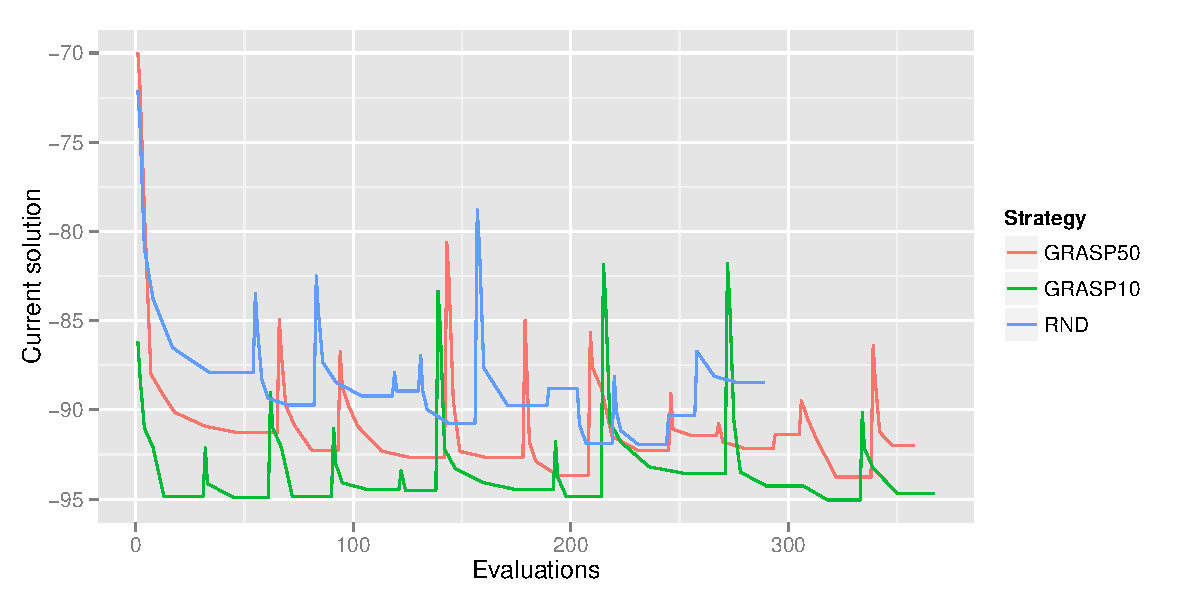
\includegraphics[width=0.45\textwidth]{./Irudiak/GRASP_vs_rndstart_4-1}
}\qquad
\subfigure[Soluziorik onena]{
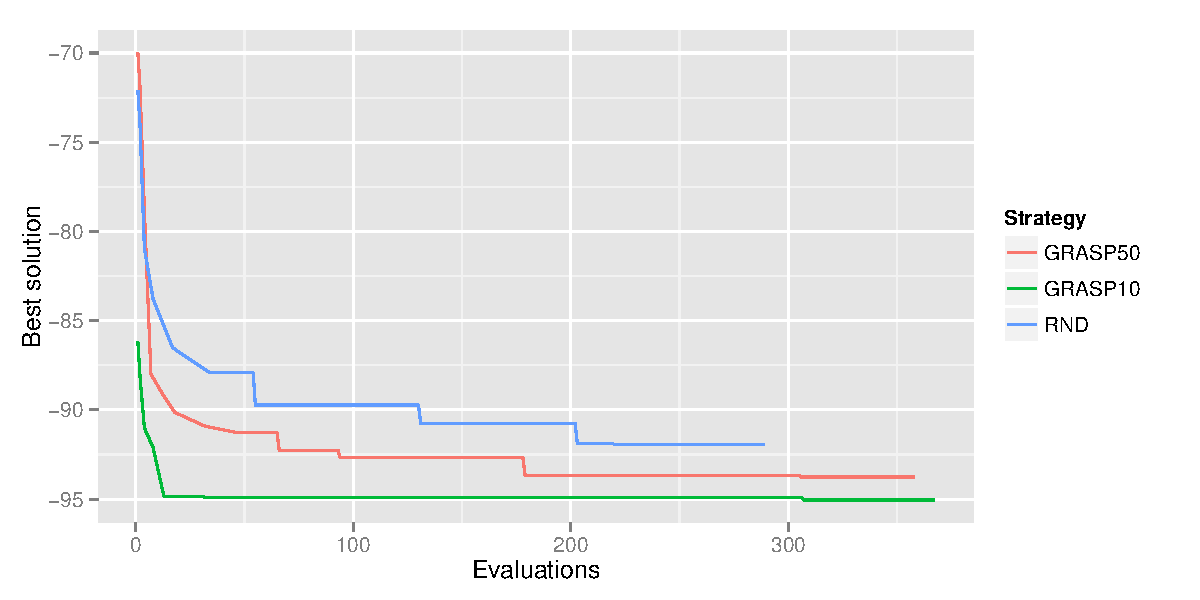
\includegraphics[width=0.45\textwidth]{./Irudiak/GRASP_vs_rndstart_4-2}
}\\

\caption{Hasieraketa anizkoitza estrategia ezberdinen konparaketa, motxilaren problema batean. Ezkerreko grafikoan uneko soluzioaren progresioa ikus daiteke. Eskumakoan, berriz, uneko soluziorik onenaren progresioa erakusten da.}\label{fig:GRASP}
\end{figure}

\ref{fig:GRASP} irudian bilaketen progresioak ikus daitezke. Ezkerreko grafikoan uneko soluzioaren eboluzioa jasotzen da. Ikusi dezakegunez, berabiaratze bakoitzean, bilaketa soluzio txarragoetatik hasten da (gorago daudenak). GRASP algoritmoan, berriz, hasierako soluzioak hobeak dira, eta baita lortzen den emaitza ere. Hori argi ikusten da eskuineko grafikoan, non uneko soluziorik onenaren eboluzioa jasotzen den.

\subsection{Inguruneko soluzioen hautaketa}

Definizioz, optimo lokalen inguruko soluzio guztiak optimo lokala bera baino okerragoak dira; hortaz, bilaketak soluzio hauetara eramaten gaituenean, ez dugu soluzio hoberik aukeratzerik eta optimizazioa trabatuta gelditzen da. Egoera hauetan, bilaketa prozesuari amaiera ez emateko, inguruneko soluzioen hautaketa estrategia alda genezake, soluzio hoberik egon ezean, helburu funtzioa hobetzen ez duten soluzioak ere onartuz. Estrategia honi esker, okerragoak diren soluzio batzuetatik pasatuz, bilaketa espazioaren eskualde berrietara ailega gintezke.

Soluzio \zkk txarragoak\skk\ aukeratzeko bi estrategia daude. Lehendabizikoan, fitness-a hobetzen ez duen soluzio bat aukeratzean, sortutako \zkk galera\skk\ kontutan hartzen da (era probabilistikoan zein deterministan egin daiteke). Algoritmorik ezagunena \textit{suberaketa estokastikoa} --\textit{simulated annealing}~\cite{kirkpatrick1983,cerny1985} ingelesez-- izenekoa da, zeinek probabilitate-banaketa parametriko bat erabiltzen duen aukeraketa egiteko. Algoritmo honetan inspiratutako beste hainbat algoritmo proposatu dira literaturan, \textit{demon algorithm}~\cite{pepper2000} eta \textit{threshold accepting}~\cite{dueck1990,moscato1990} algoritmoak, besteak beste.

Soluzio txarrak aukeratzeko bigarren estrategia mota Gloverrek 1986an proposaturiko \textit{tabu bilaketa}~\cite{glover1986} --\textit{tabu search} ingelesez-- algoritmoak erabiltzen duena da. Kasu honetan, fitness balioa hobetzen ez duten soluzioak aukeratzen dira, baina bakarrik ingurune osoan helburua hobetzen duen soluziorik ez badago. Estrategia honen arriskua dagoeneko bisitatu ditugun soluzioak berriro bisitatzea da. Hala, zikloak saihesteko, tabu bilaketak azken aldian bisitatutako soluzioak  \zkk memoria\skk\ batean gordetzen ditu.

Jarraian, bi algoritmo hauek (suberaketa simulatua eta tabu bilaketa), sakonki aztertuko ditugu.

\subsubsection{Suberaketa Simulatua}

Metalezko tresnen edo piezen sorrera prozesuan, metalek hainbat propietate gal ditzakete, euren kristal-egituran eragindako aldaketak direla eta. Propietate horiek berreskuratzeko metalurgian \zkk suberaketa\skk\ prozesua erabiltzen da; metal pieza behar adina berotzen da, gero astiro-astiro hozten uzteko. Tenperatura igotzean metalaren atomoen energia handitzen da eta, hortaz, beraien artean sortzen diren indar molekularrak apurtzeko gai dira; mugitzeko askatasun handiagoa dute, alegia. 

Metala oso azkar hozten bada --tenplatzean egiten den bezala, adibidez-- molekulak zeuden tokian \zkk izoztuta\skk\ gelditzen dira. Honek metala gogortzen du, baina hauskorragoa bihurtzen du, aldi berean. Suberatzean, berriz, metala poliki-poliki hozten da eta, ondorioz, molekulak astiro galtzen dute beraien energia --hots, abiadura--. Hozketa-abiadura motelari esker, molekulak euren kristal-egituraren \zkk kokapen optimora\skk\ joaten dira, hau da, energia minimoko kristal-egitura sortzen da.

1983an Kirkpatrick-ek~\cite{kirkpatrick1983} eta bi urte geroago Cerny-k~\cite{cerny1985}, suberaketaren prozesuan inspiratuta, optimizazio algoritmoak proposatu zituzten; Kirpatrick-ek bere algoritmoari \textit{simmulated annealing}, suberaketa simulatua, izena eman zion eta hauxe da gaur egun hedatuen dagoena.

Algoritmoaren funtzionamendua sinplea da oso. $s$ soluzio batetik txarragoa den $s^\prime$ soluzio batera mugitzeko, \zkk energia\skk\ behar dugu; behar den energia bi soluzioen ebaluazioen arteko diferentzia izango da, hau da, $\Delta E = f(s^\prime) - f(s)$. 

Energia-muga hau gainditzeko, sistemak energia behar du eta sistemaren energia \zkk tenperatura\skk k neurtuko du. Beste era batean esanda, uneoro, sistemak $T$ tenperatura izango du eta, zenbat eta tenperatura altuagoa, orduan eta errazagoa izango da energia-mugak gainditzea. Zehazki, soluzio batetik bestera mugitzeko behar den energia-muga gainditzen denetz erabakitzeko Boltzmann probabilitate-banaketan oinarritutako funtzio bat erabiltzen da:

\begin{align*}
P(\Delta E, T) = e^{-\frac{\Delta E}{T}}
\end{align*}

Ekuaziotik ondorioztatu daitekeenez, uneko soluzioa baino fitness okerragoa duen soluzio bat onartzeko probabilitatea, tenperaturarekiko proportzionala da, eta energia diferentziarekiko alderantziz proportzionala.

Aintzat hartzekoa da $\Delta E<0$ denean funtzioaren balioa 1 baino handiagoa dela. Izatez, ekuazioa bakarrik energia diferentzia positiboa denean erabiltzen da, negatiboa bada, $s^\prime$ soluzioa hobea baita eta, ondorioz, beti onartzen da.

\begin{ifalgorithm}[t]
\begin{ifpseudo}{Suberaketa Simulatua - Simulated Annealing}
\item \In\ \textit{random\_neighbor} operadorea
\item \In\ \textit{update\_temperature}, \textit{equilibrium}, \textit{stop\_condition} operadoreak
\item \Out\ $s^*$ topatutako soluziorik onena
\item $s^*=s$
\item $T=T_0$
\item \While {!\textit{stop\_condition}}
\item \T{\While{!\textit{equilibrium}}}
\item \TT{$s^\prime$ = \textit{random\_neighbor($s$)}}
\item \TT{$\Delta E = f(s^\prime)-f(s)$}
\item \TT{\If{$\Delta E < 0$}}
\item \TTT{$s=s^\prime$}
\item \TTT{\If{($f(s)<f(s^*)$)} $s^*=s$}
\item \TT{\EIf}
\item \TT{\Else}
\item \TTT{$e^{-\frac{\Delta E}{T}}$ probabilitatearekin $s=s^\prime$}
\item \T{\Done}
\item \T{\textit{T = update\_temperature(T)}}
\item \Done
\end{ifpseudo}
\caption{Suberaketa Simulatuaren sasikodea}\label{alg:SA}
\end{ifalgorithm}

Suberaketaren gakoa hozte-abiaduran datza, hau da, tenperaturaren eguneraketan. Izan ere, hasieran $T$ balio handiak erabiliko ditugu, ia edozein soluzio onartu ahal izateko, eta gero, astiro-astiro, $T$ txikiagotuko dugu, gelditzeko baldintza bete arte. \ref{alg:SA} algoritmoan suberaketa simulatuaren sasikodea ikus daiteke.

\begin{figure}[t]
\centering
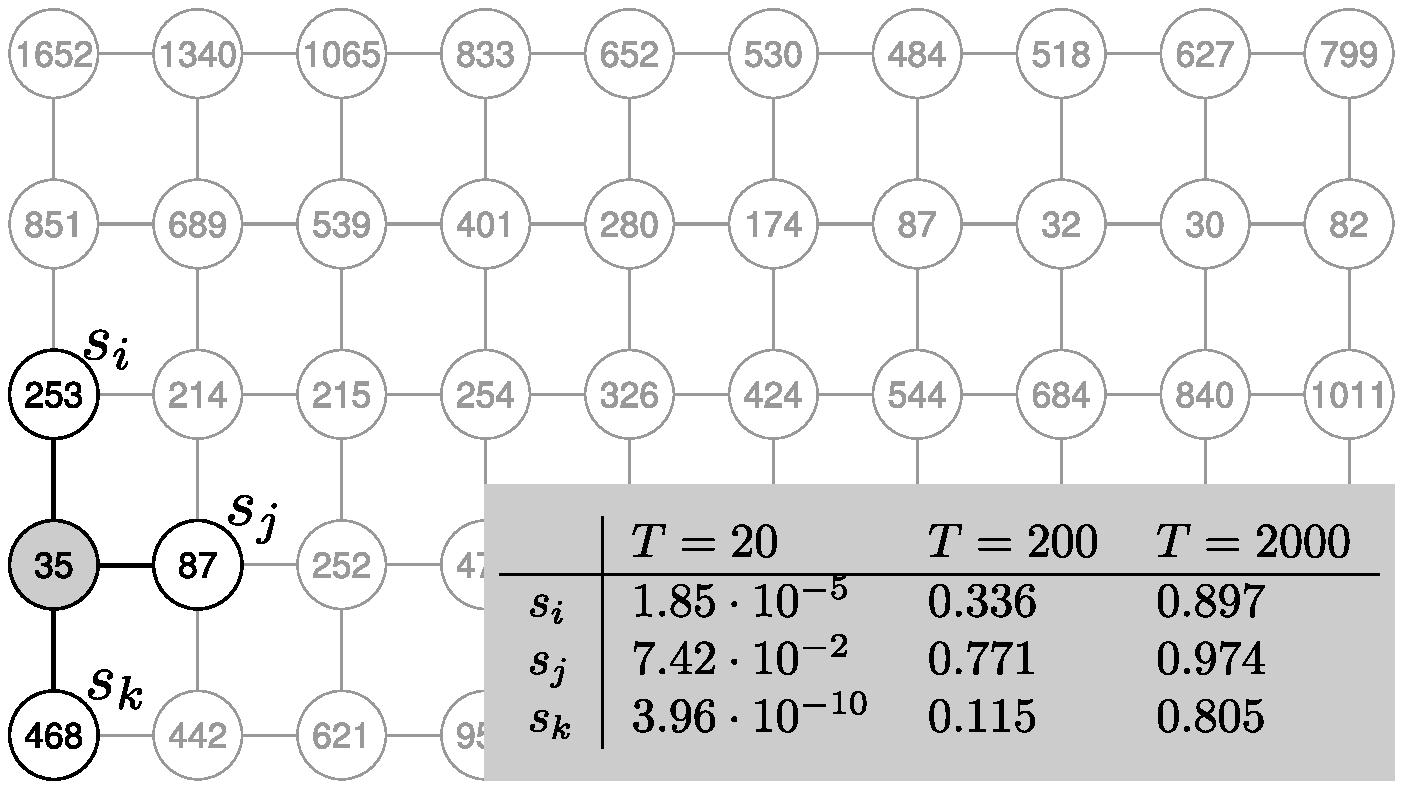
\includegraphics[width=0.66\linewidth]{./Irudiak/example_boltzman_dist}
\caption{Soluzioak onartzeko probabilitateen adibideak. Uneko soluzioa grisez nabarmendua dagoena izanik, hiru soluzio ditugu ingurunean, $s_i,s_j$ eta $s_k$. Taulak hiru tenperatura ezberdinekin soluzio bakoitza onartzeko probabilitateak jasotzen ditu. Ikus daitekeenez, tenperatura baxua denean, edozein soluzio aukeratzeko probabilitatea oso baxua da; tenperatura oso altua denean, berriz, edozein soluzio hartuta litekeena oso probablea da.}
\label{fig:example_boltzman_dist}
\end{figure}


Suberaketa simulatuan oinarritutako algoritmoak diseinatzean lau aspektu hartu behar dira kontutan:
\begin{itemize}
\item \textbf{Hasierako tenperatura} - Altuegia bada, hasierako iterazioetan \textit{random walk}, hau da, ausazko ibilbide bat jarraituko dugu; baxuegia bada, berriz, bilaketa oinarrizko bilaketa lokala bihurtuko da. \ref{fig:example_boltzman_dist} irudian adibide bat ikus daiteke. $T=20$ denean, nahiz eta fitness-en arteko diferentzia txikia izan, soluzioa onartzeko probabilitatea txikia da; $T=2000$ denean ebaluazioen arteko diferentzia handia izan arren, oso probablea da soluzioak onartzea. $T=200$ denean, berriz, optimo lokaletik atera gaitezke, probabilitate handiarekin, $s_j$ aukeratuz baina tarteko tenperatura honekin oso soluzio txarrak onartzea zaila izango da. 

Tenperatura hasieratzeko bi estrategia erabili ohi dira. Lehendabizikoa hasierako tenperatura oso altua aukeratzea da. Dibertsifikazio ikuspegitik interesgarria izan arren, estrategia honekin bilaketak asko luzatu daitezke eta konputazionalki garestia izan daiteke.  Bigarren estrategiaren funtsa bilaketa espazioaren itxura aztertzean datza, ingurunean dauden soluzioen arteko diferentziak nolakoak diren jakiteko. Informazio hau onarpen ratio edo probabilitate ezagun bat lortzeko behar dugun tenperatura finkatzeko erabili daiteke~\cite{huang1986,aarts1987}, goi eta behe mugekin egin degun antzera.


\begin{tcolorbox}
\begin{ifexample}
Demagun 10 tamainako TSP-aren instantzia bat ebatzi nahi dugula. Kostu matrizeko baliorik handiena -- hau da, bi hirien arteko distantziarik handiena -- 7.28 da. Problemarako soluzio guztietan 10 hiri izango ditugu eta, hortaz, soluzio guztien ebaluazioa matrizean dauden 10 elementuren batura izango da. Hori dela eta, $f_g=7.28 \cdot 10=78.2$ problema honen fitness-aren goi-muga bat da\footnote{Kontutan hartuz aipatutako baturan matrizeko elementuak ezin direla errepikatu, goi-muga birfindu daiteke matrizeko 10 elementurik handienak batuz}. Era berean, matrizeko distantziarik txikiena 2.5 izanik, behe-muga kalkula dezakegu: $f_b = 2.5\cdot 10$. 

Demagun, edozein soluzio aukeratzeko hasierako probabilitatea 0.75 dela. Orduan, bi muga hauek, $f_g$ eta $f_b$, hasierako tenperatura kalkulatzeko erabil ditzakegu, edozein bi soluzioen arteko fitness-en diferentzia $f_g-f_b$ baino txikiagoa izango dela baitakigu:

\begin{align*}
P=0.75= e^{-\frac{f_g-f_b}{T_0}} = e^{-\frac{78.2-25}{T_0}}\\
T_0 = -\frac{78.2-25}{\ln(0.75)} = 184.93
\end{align*}

Hasierako tenperatura 185 balioan finkatzen badugu, badakigu hasierako iterazioetan edozein soluzio aukeratzeko probabilitatea \%75 edo handiagoa izango dela.
\end{ifexample}
\end{tcolorbox}

Algoritmoaren erabilera erakusteko \ref{sec:LS_selection} ataleko adibidea erabiliko dugu (Bavariako hiriena).

\begin{knitrout}
\definecolor{shadecolor}{rgb}{1, 1, 1}\color{fgcolor}\begin{kframe}


{\ttfamily\noindent\itshape\color{messagecolor}{\#\# Processing file corresponding to instance bays29: 29 cities in Bavaria, street distances (Groetschel,Juenger,Reinelt)}}\end{kframe}
\end{knitrout}

Goiko adibidean egin dugun bezala, fitness balio maximo eta minimo posibleak kalkulatuko ditugu eta beraien arteko diferentzia hasierako tenperatura definitzeko erabiliko dugu. Horretarako, kostu matrizearen goiko triangeluanzenbaki minimoak eta maximoak bilatu beharko ditugu. Gainera, adibidean ez bezala, kasu honetan, hozketa prozesua gehiegi ez luzatzeko hasierako tenperatura kalkulatzeko diferentzia maximoaren probabilitatea 0.5-en finkatuko dugu.

\begin{knitrout}
\definecolor{shadecolor}{rgb}{1, 1, 1}\color{fgcolor}\begin{kframe}
\begin{alltt}
\hlstd{> }\hlstd{n} \hlkwb{<-} \hlkwd{ncol}\hlstd{(cost.matrix)}
\hlstd{> }\hlstd{distances} \hlkwb{<-} \hlstd{cost.matrix[}\hlkwd{upper.tri}\hlstd{(cost.matrix)]}
\hlstd{> }\hlstd{ebal.max} \hlkwb{<-} \hlkwd{sum}\hlstd{(}\hlkwd{sort}\hlstd{(distances,} \hlkwc{decreasing}\hlstd{=}\hlnum{TRUE}\hlstd{)[}\hlnum{1}\hlopt{:}\hlstd{n])}
\hlstd{> }\hlstd{ebal.min} \hlkwb{<-} \hlkwd{sum}\hlstd{(}\hlkwd{sort}\hlstd{(distances,} \hlkwc{decreasing}\hlstd{=}\hlnum{FALSE}\hlstd{)[}\hlnum{1}\hlopt{:}\hlstd{n])}
\hlstd{> }\hlstd{probability} \hlkwb{<-} \hlnum{0.5}
\hlstd{> }
\hlstd{> }\hlstd{init.t} \hlkwb{<-} \hlopt{-}\hlnum{1} \hlopt{*} \hlstd{(ebal.max} \hlopt{-} \hlstd{ebal.min)} \hlopt{/} \hlkwd{log}\hlstd{(probability)}
\hlstd{> }\hlstd{init.t}
\end{alltt}
\begin{verbatim}
## [1] 14760.21
\end{verbatim}
\end{kframe}
\end{knitrout}

\item \textbf{Oreka lortzeko iterazio kopurua} - Tenperatura eguneratzen den bakoitzean, balio honekin zenbait iterazio egiten diren -- hau da, inguruneko soluzio batzuk aztertu behar diren -- \zkk oreka\skk\ lortu arte. Behin oreka lorturik, tenperatura berriro eguneratzen da. Lehenengo pausua, beraz, oreka lortzeko behar dugun iterazio kopurua ezartzea da. Ohikoena inguruneko tamainaren araberako iterazio kopuru bat finkatzea da. Horretarako, $\rho$ parametroa erabiliko dugu (0 eta 1 tartean hartuko ditu balioak), tenperatura bakoitzeko $\rho|N(s)|$ soluzio ebaluatuko ditugularik. Aurreko atalean azaldu dugun bezala, $|N(s)|$-k uneko soluzioaren bizilagun kopurua adierazten du.

Beste estrategia batzuek, tenperatura bakoitzeko iterazio kopuru desberdina ezartzea proposatzen dute.  Adibide gisa, tenperatura soluzio berri bat onartzen dugun bakoitzean alda dezakegu; Soluzioen onarpena haien fitness balioaren araberako probabilitate balio baten menpekoa denez, batzuetan ebaluatzen dugun lehendabiziko soluzioa onartuko dugu eta, bestetan, hainbat soluzio probatu beharko ditugu, bat onartu arte. Kasu honetan, beraz, iterazio kopurua aldakorra da. 


\item \textbf{Tenperatura jaitsieraren abiadura} - Hau da, ziurrenik, algoritmoaren elemeturik garrantzitsuena. Hainbat formula erabil daitezke tenperatura eguneratzeko. Hona hemen batzuk:
  \begin{itemize}
  \item \textit{Lineala}: $T_i=T_0 - i\beta$, non $T_i$ $i$. iterazioko tenperatura den. Eguneraketa mota honetan tenperatura beti positiboa izan behar dela kontrolatu behar dugu, ekuazioak tenperatura negatiboak itzuli baititzake.
  \item \textit{Geometrikoa}: $T_i = \alpha T_{i-1}$. $\alpha \in (0,1)$ abiadura kontrolatzen duen parametroa da eta, ohikoena, 0.5 eta 0.99 tarteko balio bat aukeratzea da.
  \item \textit{Logaritmikoa}: $T_i=\frac{T_0}{log(i)}$. Abiadura hau oso motela da eta, nahiz eta praktikan oso erabilgarria ez izan, interes teorikoa du suberaketa simulatu algoritmoaren konbergentzia demostratuta baitago ekuazio honekin.
\end{itemize}
Funtzio guzti hauek monotonoak dira, hau da, iterazio bakoitzean tenperatura beti jaisten da. Edonola ere, problema batzuetan funtzio ez-monotonoek hobeto funtziona dezakete\footnote{Tenperatura igotzen denean dibertsifikazioan gailentzen da; tenperatura jaistean, berriz, areagotze prozesua indartzen da. Hau kontutan hartuz, funtzio ez-monotonoak dibertsifikazio/areagotze prozesuen arteko oreka kontrolatzeko erabil daitezke}.

\item \textbf{Algoritmoa gelditzeko irizpidea} - Aurreko puntuan ikusi dugun legez, iterazioak aurrera egin ahala tenperatura zero baliora hurbiltzen da baina, kasu gehienetan, ez da inoiz heltzen. Honek esan nahi du beti optimo lokaletatik ateratzeko aukera izango dugula, probabilitate oso txikiarekin bada ere. Hori dela eta, algoritmoa gelditzeko baldintzaren bat definitu beharko dugu. Irizpide hedatuena tenperatura minimo bat finkatzea da; bestela, denbora edota helburu funtzioaren ebaluazio kopuru maximo bat ere finka ditzakegu.
\end{itemize}

Suberaketa simulatuaren erabilera erakusteko Bavierako TSP adibidearekin jarraituko dugu. Algoritmoa \code{simulatedAnnealing} funtzioak inplementatzen du. Funtzio honek, ohiko argumentuez gain, beste zenbait parametro berezi ditu:

\begin{itemize}
\item \code{cooling.scheme} - Tenperaturaren eguneraketa funtzioa. Funtzioak uneko tenperatura jasoko du argumentu gisa eta hurrengo tenperatura itzuliko du.
\item \code{initial.temperature} - Hasierako tenperatura.
\item \code{final.temperature} - Amaierako tenperatura. Hau algoritmoa gelditzeko irizpidea definitzeko erabiltzen da.
\item \code{eq.criterion} - Oreka baldintza zeren araberakoa den adierazten duen \textit{string} motako parametro bat da. Bi balio posible har ditzake, \code{\tq evaluations\tq} eta \code{\tq acceptances\tq}. Lehenengoa erabiltzen bada, oreka baldintza ebaluazio kopuru jakin batera iristean beteko da. Bigarren kasuan, ostera, uneko soluzioaren fitness-a hobetzen ez duten soluzio kopuru finko bat onartzen denean beteko da.
\item \code{eq.value} - \code{eq.criterion} parametroa zehaztuko duen ebaluazio edo onarpen kopurua.
\end{itemize}

 Hasierako tenperatura kalkulatu dugu, baina ez amaierakoa. Aukera posible bat, ausaz soluzioak sortu eta beraien fitnessen arteko diferentzien behe-muga kalkulatzea da.

Estrategia hau gauzatzeko 500 ausazko soluzio sortuko eta ebaluatuko ditugu. Gero, edozein bi soluzioen arteko diferentzia balio absolutuan konputatuko dugu. Azkenik, 0 ez diren diferentzien artean txikiena hartuko dugu behe-muga gisa.

\begin{knitrout}
\definecolor{shadecolor}{rgb}{1, 1, 1}\color{fgcolor}\begin{kframe}
\begin{alltt}
\hlstd{> }\hlstd{rep} \hlkwb{<-} \hlnum{500}
\hlstd{> }\hlstd{rnd.eval} \hlkwb{<-} \hlkwd{sapply} \hlstd{(}\hlnum{1}\hlopt{:}\hlstd{rep,}
\hlstd{+ }                    \hlkwc{FUN}\hlstd{=}\hlkwa{function}\hlstd{(}\hlkwc{x}\hlstd{) \{}
\hlstd{+ }                      \hlkwd{return}\hlstd{(tsp.babaria}\hlopt{$}\hlkwd{evaluate}\hlstd{(}\hlkwd{randomPermutation}\hlstd{(n)))}
\hlstd{+ }                    \hlstd{\})}
\hlstd{> }
\hlstd{> }\hlstd{aux} \hlkwb{<-} \hlkwd{lapply}\hlstd{(}\hlnum{2}\hlopt{:}\hlstd{rep,}
\hlstd{+ }              \hlkwc{FUN}\hlstd{=}\hlkwa{function}\hlstd{(}\hlkwc{i}\hlstd{) \{}
\hlstd{+ }                \hlkwd{return}\hlstd{(}\hlkwd{cbind}\hlstd{(i}\hlopt{-}\hlnum{1} \hlstd{, i}\hlopt{:}\hlstd{rep))}
\hlstd{+ }              \hlstd{\})}
\hlstd{> }\hlstd{pairs} \hlkwb{<-} \hlkwd{do.call}\hlstd{(rbind, aux)}
\hlstd{> }
\hlstd{> }\hlstd{diffs} \hlkwb{<-} \hlkwd{apply}\hlstd{(pairs,} \hlkwc{MARGIN}\hlstd{=}\hlnum{1}\hlstd{,}
\hlstd{+ }               \hlkwc{FUN}\hlstd{=}\hlkwa{function}\hlstd{(}\hlkwc{p}\hlstd{) \{}
\hlstd{+ }                 \hlkwd{return}\hlstd{(}\hlkwd{abs}\hlstd{(rnd.eval[p[}\hlnum{1}\hlstd{]]} \hlopt{-} \hlstd{rnd.eval[p[}\hlnum{2}\hlstd{]]))}
\hlstd{+ }               \hlstd{\})}
\hlstd{> }\hlstd{min.delta} \hlkwb{<-} \hlkwd{min}\hlstd{(}\hlkwd{subset}\hlstd{(diffs, diffs} \hlopt{!=} \hlnum{0}\hlstd{))}
\hlstd{> }\hlstd{min.delta}
\end{alltt}
\begin{verbatim}
## [1] 1
\end{verbatim}
\end{kframe}
\end{knitrout}

Fitness balioen diferentzia horri probabilitate txiki bat esleituz, tenperatura minimoa kalkula dezakegu.

\begin{knitrout}
\definecolor{shadecolor}{rgb}{1, 1, 1}\color{fgcolor}\begin{kframe}
\begin{alltt}
\hlstd{> }\hlstd{probability} \hlkwb{<-} \hlnum{0.1}
\hlstd{> }\hlstd{final.t} \hlkwb{<-} \hlopt{-}\hlstd{min.delta} \hlopt{/} \hlkwd{log}\hlstd{(probability)}
\hlstd{> }\hlstd{final.t}
\end{alltt}
\begin{verbatim}
## [1] 0.4342945
\end{verbatim}
\end{kframe}
\end{knitrout}

Gauza berdina egin dezakegu tenperatura maximoa kalkulatzeko, lehen kalkulatutako goi-mugarekin alderatu ahal izateko.

\begin{knitrout}
\definecolor{shadecolor}{rgb}{1, 1, 1}\color{fgcolor}\begin{kframe}
\begin{alltt}
\hlstd{> }\hlstd{init.t}
\end{alltt}
\begin{verbatim}
## [1] 14760.21
\end{verbatim}
\begin{alltt}
\hlstd{> }\hlstd{max.delta} \hlkwb{<-} \hlkwd{max}\hlstd{(diffs)}
\hlstd{> }\hlstd{probability} \hlkwb{<-} \hlnum{0.5}
\hlstd{> }\hlstd{init.t} \hlkwb{<-} \hlopt{-}\hlstd{max.delta} \hlopt{/} \hlkwd{log}\hlstd{(probability)}
\hlstd{> }\hlstd{init.t}
\end{alltt}
\begin{verbatim}
## [1] 3794.288
\end{verbatim}
\end{kframe}
\end{knitrout}

Ikus daitekeen bezala, simulazio bitartez kalkulatutako diferentzietan oinarritzen bagara, hasierako tenperatura askoz ere txikiagoa da, teorikoki kalkulatutako goi-muga laginketan lortu ditugun diferentziak baino handiagoa delako.

Informazio guztiarekin funtzioaren argumentuak pausuz pausu munta ditzakegu. Ingurunea definitzeko, ondoz-ondoko trukaketak erabiliko ditugu eta bilaketa ausazko soluzio batetik abiatuko dugu.

\begin{knitrout}
\definecolor{shadecolor}{rgb}{1, 1, 1}\color{fgcolor}\begin{kframe}
\begin{alltt}
\hlstd{> }\hlkwd{set.seed}\hlstd{(}\hlnum{90}\hlstd{)}
\hlstd{> }
\hlstd{> }\hlstd{args}\hlopt{$}\hlstd{evaluate}         \hlkwb{<-} \hlstd{tsp.babaria}\hlopt{$}\hlstd{evaluate}
\hlstd{> }\hlstd{args}\hlopt{$}\hlstd{initial.solution} \hlkwb{<-} \hlkwd{randomPermutation}\hlstd{(n)}
\hlstd{> }\hlstd{args}\hlopt{$}\hlstd{neighborhood}     \hlkwb{<-} \hlkwd{swapNeighborhood}\hlstd{(args}\hlopt{$}\hlstd{initial.solution)}
\end{alltt}
\end{kframe}
\end{knitrout}

Hozketa funtzioa sortzeko \code{geometricCooling} funtzioa erabiliko dugu --hozketa geometrikoa inplementatzen duena--. Funtzio honi hasierako eta amaierako tenperaturak eman behar dizkiogu. Horrez gain, hasierako tenperaturatik amaierakora zenbat eguneraketa behar diren ere adierazi beharko diogu.

\begin{knitrout}
\definecolor{shadecolor}{rgb}{1, 1, 1}\color{fgcolor}\begin{kframe}
\begin{alltt}
\hlstd{> }\hlstd{steps} \hlkwb{<-} \hlnum{20}
\hlstd{> }\hlstd{args}\hlopt{$}\hlstd{cooling.scheme}      \hlkwb{<-} \hlkwd{geometricCooling}\hlstd{(init.t, final.t, steps)}
\hlstd{> }\hlstd{args}\hlopt{$}\hlstd{initial.temperature} \hlkwb{<-} \hlstd{init.t}
\hlstd{> }\hlstd{args}\hlopt{$}\hlstd{final.temperature}   \hlkwb{<-} \hlstd{final.t}
\end{alltt}
\end{kframe}
\end{knitrout}

Eguneraketa funtzioari tenperatura bat emanik, hurrengo tenperatura emango digu.

\begin{knitrout}
\definecolor{shadecolor}{rgb}{1, 1, 1}\color{fgcolor}\begin{kframe}
\begin{alltt}
\hlstd{> }\hlstd{init.t}
\hlstd{> }\hlstd{next.t} \hlkwb{<-} \hlstd{args}\hlopt{$}\hlkwd{cooling.scheme}\hlstd{(init.t)}
\hlstd{> }\hlstd{next.t}
\hlstd{> }\hlstd{next.t} \hlkwb{<-} \hlstd{args}\hlopt{$}\hlkwd{cooling.scheme}\hlstd{(next.t)}
\hlstd{> }\hlstd{next.t}
\end{alltt}
\end{kframe}
\end{knitrout}

Oreka egoera, soluzio berrien ebaluazio kopuru baten arabera kontsideratuko dugu. Zehazki, 10 bider ingurunearen tamaina (hiri kopurua) izango da.

\begin{knitrout}
\definecolor{shadecolor}{rgb}{1, 1, 1}\color{fgcolor}\begin{kframe}
\begin{alltt}
\hlstd{> }\hlstd{args}\hlopt{$}\hlstd{log.frequency} \hlkwb{<-} \hlnum{10}
\hlstd{> }\hlstd{args}\hlopt{$}\hlstd{eq.criterion}  \hlkwb{<-} \hlstr{"evaluations"}
\hlstd{> }\hlstd{args}\hlopt{$}\hlstd{verbose}       \hlkwb{<-} \hlnum{FALSE}
\end{alltt}
\end{kframe}
\end{knitrout}

Amaitzeko, algoritmoa exekutatzen dugu.





\begin{figure}[t]
\centering
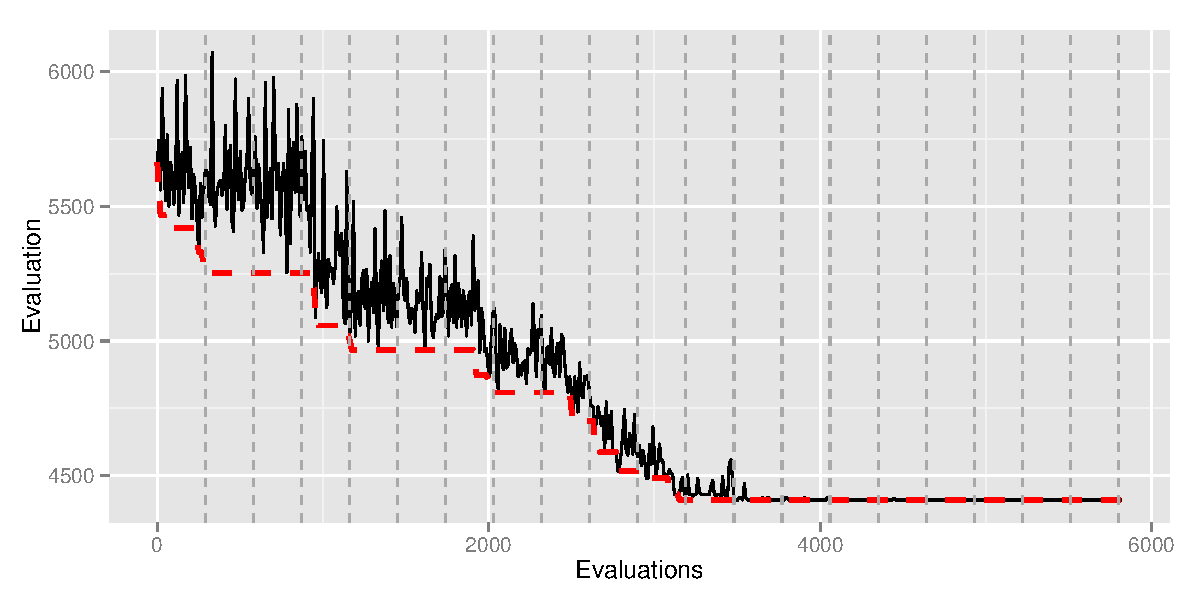
\includegraphics[width=0.75\linewidth]{./Irudiak/TSP_SA_7-1}
\caption{Simulated annealing algoritmoaren progresioa TSP problema batean. Marra jarraikiak uneko soluzioaren progresioa adierazten du eta etenak, berriz, arkitutako soluziorik onena. Marra bertikalek teneraturaren aldaketak erakusten dituzte.}
\label{fig:SA}
\end{figure}

Bilaketaren eboluzioa \ref{fig:SA} irudian dago jasota. Irudiak, uneko soluzioaren eta soluziorik onenaren progresioak erakusten ditu (beltzez eta gorriz, hurrenez hurren). Grafikoan marra bertikal bat agertzen denean, tenperatura aldaketa bat egon dela esan nahi du. Uneko soluzioaren eboluzioan ikus daiteke ebaluazioa, hasieran, oso aldakorra dela. Hau tenperaturaren eraginaren ondorioz da, tenperatura altuak soluzio txarrak aukeratzeko probabilitatea handitzen baitu. Hozketa prozesuaren zehar, tenperatura jaisten den heinean, soluzio txarrak onartzeko probabilitatea txikitu egiten da eta, ondorioz, soluzioen arteko aldakortasuna murriztu egiten da. Amaieran, tenperatura oso txikia denean, ia ezinezkoa da soluzio okerragoak onartzea eta, hortaz, uneko soluzioa ez da ia aldatzen.

 Grafikan ere ikus daiteke algoritmoak oso azkar konbergitzen duela. Bilatu duen soluzioa optimo globala bada, honek esan nahi du algoritmoak oso ondo funtzionatu duela. Aldiz, tenperatura azkarregi jeitsi badugu, posible da algoritmoak optimo globalaren ingurua ez den leku batean intensifikatu izana bilaketa. Hori ez gertatzeko, eta algoritmoak gehiago dibertsifikatzeko, azken tenperatura handiagoa jarri daiteke. 

Ikusitako algoritmoetan soluzioen onarpena probabilistikoa da; alabaina, suberaketa simulatuaren kontzeptua era deterministan ere inplementa daiteke. Honen adibidea da Deabru Algoritmoa~\cite{pepper2000} -- \textit{Demon Algorithm}, ingelesez --. Hasiera batean Creutz-ek  simulazio molekularrak egiteko proposatu zuen algoritmo hau, baina optimizazio problemak ebazteko ere egoki daiteke. 

Algoritmoan soluzioak onartuko direnetz erabakitzeko, tenperatura erabili beharrean \zkk deabru\skk\ bat erabiltzen da; deabru honek uneoro $E_D$ energia kopurua dauka. Soluzio bakoitza aztertzerakoan, subaeraketa simulatuan legez, $\Delta E$ kalkulatzen da eta, une horretan $\Delta E>E_D$ bada, soluzioa onartzen da. Gainera, suberaketa simulatuan bezala, $\Delta E<0$ denean ere soluzioa onartu egiten da. 

Algoritmoaren gakoa deabruaren energia eguneratzean datza; soluzio bat onartzen den bakoitzean, deabruaren energia $E_D + \Delta E$ izatera pasatzen da, hau da, \zkk sistemaren\skk\ energia aldaketa deabruak jasotzen du. Onartutako soluzioa hobea denean, deabruak energia irabazten du eta, okerragoa denean, berriz, energia galtzen du -- nahiko energia baldin badu betiere --. Algoritmo honen abantaila sinpletasuna da, Boltzmann distribuzioa ebaluatzeko beharrik ez baitago.

\subsubsection{Tabu bilaketa}

Tabu bilaketa -- \textit{tabu search}, inglesez -- izango da, ziurrenik , bilaketa lokalaren aldaerarik hedatuena. Duen eraginkortasuna eta sinpletasuna dela eta, optimizazio konbinatorioan asko erabiltzen da eta, zenbait problematan, emaitza onenak ematen dituen metaheuristikoa da.

1977an proposatu zen lehenengo aldiz eta optimo lokaletan trabaturik ez geratzeko, bilaketa soluzio okerragoetara bideratzea baimentzen du. Estrategia hau hutsean erabiliz gero, prozesua amaigabeko ziklo batean sartzeko arriskua dago, egindako bidea behin eta berriro errepikatzeko aukera baitago. Beraz, arazo hau saihesteko, tabu bilaketak, bisitatutako soluzioen historikoa gordetzen du.

\begin{ifalgorithm}[t]
\begin{ifpseudo}{Tabu Bilaketa}
\item \In\ \textit{intensify} eta \textit{diversify} operadoreak
\item \In\ \textit{intensify\_condition}, \textit{diversify\_condition} eta \textit{stop\_condition} baldintzak
\item \In\ $\cal N$ ingurune operadorea eta $s_0$ hasierako soluzioa
\item \Out\ $s^*$ topatutako soluziorik onena
\item $s^*=s_0$
\item $s = s_0$
\item Hasieratu tabu zerrenda, epe erdiko memoria eta epe luzeko memoria
\item \While {!\textit{stop\_condition}}
\item \T{Topatu ${\cal N}(s)$-n dagoen soluzio onargarririk onena $s^\prime$}
\item \T{$s = s^\prime$}
\item \T{Eguneratu tabu lista}
\item \T{\If{\textit{intensify\_condition}}}
\item \TT{\textit{intensify}}
\item \T{\EIf}
\item \T{\If{\textit{diversify\_condition}}}
\item \TT{\textit{diversify}}
\item \T{\EIf}
\item \Done
\end{ifpseudo}
\caption{Tabu bilaketaren sasikodea}\label{alg:tabu}
\end{ifalgorithm}


Oinarrizko tabu bilaketa, bilaketa lokal gutiziatsuan oinarritzen da, baina \zkk tabu zerrenda\skk\ deituriko bisitatutako soluzioen multzoa gordeko da uneoro. Urrats bakoitzean tabu ez diren -- bideragarriak diren, alegia -- inguruneko soluzioetatik onena aukeratuko dugu, helburu funtzioa hobetzen duen ala ez kontutan hartu barik. Tabu ez diren soluzioak bakarrik hartzen ditugunez aintzat, ez da ziklorik sortuko.

Alabaina, bisitatutako soluzio guztiak gordetzen dituen zerrenda mantentzea ez da bideragarria; hori dela eta, tabu zerrendan bisitatutako azkeneko soluzioak bakarrik gordeko ditugu. Algoritmoaren iterazio bakoitzean, aukeratutako soluzioa tabu zerrendan sartuko da, eta zerrendatik soluzio bat aterako da -- tabu zerrendak FIFO pilak dira, hau da, sartzen lehendabizikoa den elementua ateratzen ere lehendabizikoa izango da--. Bisitatutako azken soluzioak bakarrik gordetzen direnez tabu zerrendari epe laburreko memoria ere deitzen zaio.

Bigarren estrategia mota honekin, tabu zerrendaren tamaina $k$ bada $k$ tamainako zikloak ekiditeko gai izango gara. Edonola ere, eraginkortasuna dela eta, soluzio osoak maneiatzeak kostu handia ekar dezake. Hori dela eta, aukera egokiagoak ere aurki ditzakegu literaturan, soluzioen atributu batzuk soilik gordetzea, adibidez. Atributuak soluzioen zatiak, ezaugarriak, edo soluzioen arteko desberdintasunak izan ohi dira. Hauek, ebazten ari garen problemaren menpekoak dira eta, hortaz, aukera ugari proposatu daitezke, kasu bakoitzerako tabu lista eredu desberdin bat inplementatuz. Ikus dezagun adibide bat.

\begin{tcolorbox}
\begin{ifexample}
Demagun permutazioetan oinarritutako problema batean tabu bilaketa bat inplementatu nahi dugula. Bilaketa lokalak {\em 2-opt} ingurunea erabiltzen badu, soluzio batetik bestera mugitzeko $i$ eta $j$ posizioak trukatuko ditugu. Era honetan, tabu zerrendan trukatzen ditugun bi posizioak gorde ditzakegu, alderantzizko trukaketa tabu bihurtuz. Esate baterako, uneko soluzioa $13245$ bada eta $31245$ soluziora mugitzen bagara, hurrengo urratsetan lehenengo eta bigarren posizioak trukatzea debekatua izango dugu. Problemaren arabera, beste irizpide batzuk erabil genitzake. Adibide gisa, lehenengo posizioan $1$a eta bigarrenean $3$a egotea debekatu genezake.
\end{ifexample}
\end{tcolorbox}

Soluzioen atributuak erabiltzen ditugunean memoria gutxiago behar dugu eta, hortaz, tabu zerrenda handiagoak erabil ditzakegu; edonola ere, kontuan eduki behar da estrategia honekin tabu zerrenda baino txikiagoak diren zikloak ager daitezkeela. Horrez gain, diseinatutako atributuak oso zehatzak izan behar dira, bisitatu gabeko soluzio onak baztertu ez ditzagun. Ildo honetan \textit{aspiration criteria} deritzen irizpideak erabili ohi dira bilaketa prozesuan tabu  diren soluzioak onartzeko. Esate baterako, uneko soluziotik, tabu den mugimendu bat erabiliz orain arte topatutako soluziorik onena topatzen badugu, soluzio horretara bai pasatuko gara.

Tabu zerrendaren tamainak, tabu bilaketaren portaera definitzen du; txikia baldin bada, espazioko eremu txikietan zentratuko da; handia bada, berriz, algoritmoak eremu zabalagoetara bideratuko du bilaketa, soluzio asko tabu izango baitira. Ohikoena, lista tamaina aldakor bat erabiltzea da, algoritmoaren portaera kasu bakoitzeko beharretara egokitu ahal izateko.

Tabu zerrendaz gain, bestelako aukera konplexuagoak ere proposatu dira. Epe motzeko memoria erabiltzeaz gain, bilaketa prozesuan zehar jasotako informazioa ere oso baliotsua izan daiteke algoritmoa gidatzeko. Informazio hau epe erdiko edota epe luzeko memorian gorde daiteke. Lehendabiziko kasuan soluzio onenen informazioa bakarrik gordeko dugu, bilaketa areagotzeko asmoarekin. Bigarren kasuan, berriz, bilaketa osoan zehar soluzioen osagaien frekuentziak gordeko ditugu; frekuentzia hauek bisitatu ez ditugun eremuei atzemateko erabil daitezke -- hau da, bilaketa dibertsifikatzeko --.


\begin{tcolorbox}
\begin{ifexample}
TSP-rako soluzioak eraikitzeko, hiri bakoitzetik zein hirira mugituko garen erabaki behar dugu. Algoritmo eraikitzaile tipikoan, erabaki hori kostu matrizea begiratuz hartzen da, uneko hiritik bisitatu gabeko hirietatik gertuen dagoena aukeratuz. Era berean, epe erdiko eta epe luzeko memoriak matrize karratu batean inplementa ditzakegu. Matrize hauetan, bisitatutako zenbat soluzioetan $i$ hiritik $j$ hirira joaten garen gordeko dugu. Epe erdiko memorian azken $k$ soluzio onenen informazioa bakarrik gordeko dugu, areagotze prozesuan gehien erabili direnak finkatzeko eta bilaketa falta diren loturetan zentratzeko. Epe luzeko memorian, berriz, bisitatu ditugun soluzio guztien informazioa gordeko dugu. Era honetan, bilaketa esploratu gabeko eremuetara eraman nahi badugu, gutxien erabilitako loturak erabiliz soluzioak sor ditzakegu, bilaketa prozesua bertatik abiatzeko.
\end{ifexample}
\end{tcolorbox}


\subsection{Optimizazio problemen \zkk itxura\skk aldaketa}

Bilaketa lokalean uneko soluziotik honen inguruan dagoen soluzio batera mugitzen gara beti, hau da, soluzio bakoitzetik soluzio kopuru mugatu batetara mugi gaitezke soilik. Hori dela eta, bilaketa espazioa grafo baten bidez adieraz daiteke, non erpinak soluzioak diren eta ertzek mugimendu posibleak adierazten dituzten; \ref{fig:local_optimum} irudiak horrelako grafo bat adierazten du.

Bilaketa espazioaren definizioari soluzioen ebaluazioa gehitzen badiogu, optimizazio problemaren \zkk itxura\skk\ -- \textit{landscape}-a, ingelesez -- daukagu. Problemaren itxuraren eragina berebizikoa da algoritmoen performantzian eta, beraz, algoritmoak diseinatzerakoan kontuan hartu beharreko elementua da. Zentzu horretan, kontuan hartu behar da problema motaren arabera ez ezik, \textit{landscape}-a  instantzia konkretuaren arabera aldatzen dela. Optimizazio problemen "itxuraren" idea intuikorra, gailurrez, mendikatez eta bailarez osatutako paisaia baten ilustrazioa da, non gailurrek optimo lokalak errepresentatzen dituzten eta gailurrik altuena optimo globala den. Gailur baten erakarpen-arroa, mendi osoa da, oinarritik gailurrera. Intuitiboki, zenbat eta gailur gehiago, orduan eta zailagoa izango da instantzia baten optimo globalera heltzea bilaketa lokalean oinarritutako algoritmo batekin.

Soluzio bakarrean oinarritzen diren algoritmoekin amaitzeko, bilaketa prozesuan zehar, \textit{landscape}-a eraldatzen dituzten algoritmoak aztertuko ditugu. Zehazki, bi algoritmo ikusiko ditugu. Lehenengoak, VNS-ak, ingurune definizio ezberdinak erabiltzen ditu optimo lokaletatik ateratzeko. Bigarrenak, berriz, helburu funtzio berriak sortzen ditu optimo lokalen kopurua murrizteko.

\subsubsection{Variable Neighborhood Search algoritmoa}

Bilaketa lokalean optimo lokal batean trabaturik gelditzen gara, definizioz bere ingurunean helburu funtzioa hobetzen duen soluziorik ez dagoelako. Baina, zer gertatuko litzateke ingurunearen definizioa aldatuko bagenu?. Adibide gisa, demagun optimizazio problema batean soluzioak permutazioen bidez kodetzen ditugula. Bilaketa lokala aplikatzeko \textit{2-opt} operadorea erabiliko dugu -- hau da, \textit{swap} eragiketan oinarritutako ingurunea --. Izan bedi $1432$ soluzioa, ingurune eta problema honetarako optimo lokala dena. Definizioz, soluzio honen edozein bi posizio trukatuz lortutako soluzioak okerragoak izango dira. Alabaina, txertaketan oinarritzen den ingurunea erabiliz \textit{2-opt} ingurunean ez dauden soluzioak lor ditzakegu -- lehenengo elementua azken elementuaren ostean txertatuz lortzen den $4321$ soluzioa, esate baterako --. Beraz, gerta daiteke \textit{2-opt} ingururako optimo lokala den gure soluzioa txertaketak definitzen duen ingurunerako optimoa ez izatea.

Ideia hau \textit{Variable Neighborhood Descent} (VND) algoritmoan erabiltzen da bilaketa lokala optimo lokaletan trabaturik geratzea ekiditeko. \ref{alg:VND} algoritmoan VND-aren sasikodea ikus daiteke. 

\begin{ifalgorithm}[t]
\begin{ifpseudo}{VND algoritmoaren sasikodea}
\item \In\ $\mathbf{\cal N} = \{{\cal N}_1,\ldots,{\cal N}_k\}$ ingurune funtzioak
\item \In\ $s$ hasierako soluzioa
\item  $i=1$
\item  $s^* = s$
\item \While {$i\leq k$} \Do
\item \T{Bilatu $s^\prime$, ${\cal N}_i(s^*)$ inguruneko soluziorik onena}
\item \T{\If{$f(s^\prime<f(s^*)$}}
\item \TT{$s^*=s^\prime$}
\item \TT{$i=1$}
\item \T{\Else}
\item \TT{$i=i+1$}
\item \T{\EIf}
\item \Done
\end{ifpseudo}
\caption{VND algoritmoaren sasikodea}\label{alg:VND}
\end{ifalgorithm}

Algoritmoan ikusten den bezala, VND-an ingurune funtzio bakarra izan beharrean hauen multzo bat dago. Lehenengo ingurunea erabiliz, uneko soluzioaren ingurunea arakatu eta soluzio onena aukeratuko dugu. Inguruneko soluzio guztiak okerragoak direnean -- topatutako soluzioa uneko ingurunerako optimo lokala bada, alegia -- hurrengo ingurune definiziora pasatuko gara; honela, ingurune funtzio guztiak erabili arte. Gainera, iterazio bakoitzean, inguruneko soluzio berri batera pasatzen garenean, berriro ere hasierako ingurune definiziora itzuliko gara.

Bilaketa amaitzeko baldintza kontutan hartuz, algoritmo honek itzultzen duen soluzioa \textit{ingurune definizio guztietarako optimo lokala} izango da.

\textit{Variable Neighborhood Search} algoritmoa VND-aren hedapen bat da, non iterazio bakoitzean, uneko ingurune definizioa erabiliz, bilaketa lokala amaiera arte eramaten den. Hau da, fitness-a hobetzen duen soluzio bat topatu arren, uneko ingurune definizioa mantentzen dugu optimo lokal batera heldu arte. Behin optimo lokal batera heldutakoan, hurrengo ingurune definizioa erabiltzera pasatuko gara, VND-an legez, lortutako soluzioa ingurune guztietarako optimo lokala izan arte. \ref{alg:VNS} algoritmoak VNS-aren sasikodea erakusten du.

\begin{ifalgorithm} [t]
\begin{ifpseudo}{Oinarrizko VNS algoritmoaren sasikodea}
\item \In\ \textit{local\_search} bilaketa algoritmoa
\item \In\ $\mathbf{\cal N} = \{{\cal N}_1,\ldots,{\cal N}_k\}$ ingurune funtzioak
\item \In\ $s$ hasierako soluzioa
\item  $i=1$
\item  $s^* = s$
\item \While {$i\leq k$} \Do
\item \T{Aukeratu ausaz soluzio bat $s^\prime\in {\cal N}_i(s^*)$}
\item \T{$s^{\prime\prime} = $\textit{local\_search}($s^*$,${\cal N}_i$)}
\item \T{\If{$f(s^{\prime\prime})<f(s^*)$}}
\item \TT{$s^*=s^{\prime\prime}$}
\item \TT{$i=1$}
\item \T{\Else}
\item \TT{$i=i+1$}
\item \T{\EIf}
\item \Done
\end{ifpseudo}
\caption{VNS algoritmoaren sasikodea}\label{alg:VNS}
\end{ifalgorithm}


\subsection{\textit{Smoothing} algoritmoak}

Optimizatu behar dugun funtzioak optimo lokal asko dituenean, bilaketa lokalak ez dira oso metodo egokiak, globala ez den optimo batean trabaturik gelditzeko probabilitatea oso altua delako. Leuntze-metodoekin -- \textit{smoothing methods}, ingelesez -- iterazio bakoitzean jatorrizko helburu funtzioa eraldatu -- leundu -- egiten da, optimo lokal kopurua gutxitzeko asmoz; eta helburu funtzio berria erabiliz, bilaketa lokala aplikatzen da. Bilaketa trabaturik geratzen denean -- optimo lokal batean --, helburu funtzioa berriro aldatzen da, aurreko iterazioan baino gutxiago leunduz. Helburu funtzio berri honekin eta aurreko iterazioan lortutako optimoarekin, bilaketa lokala aplikatzen da, optimo berri bat lortuz. 

Iterazioz iterazio leuntze-maila geroz eta txikiagoa bihurtuz, azken iterazioan problemaren jatorrizko helburu funtzioa erabiliko dugu, problemarako soluzioa topatzeko. 


\begin{figure}[t]
\centering
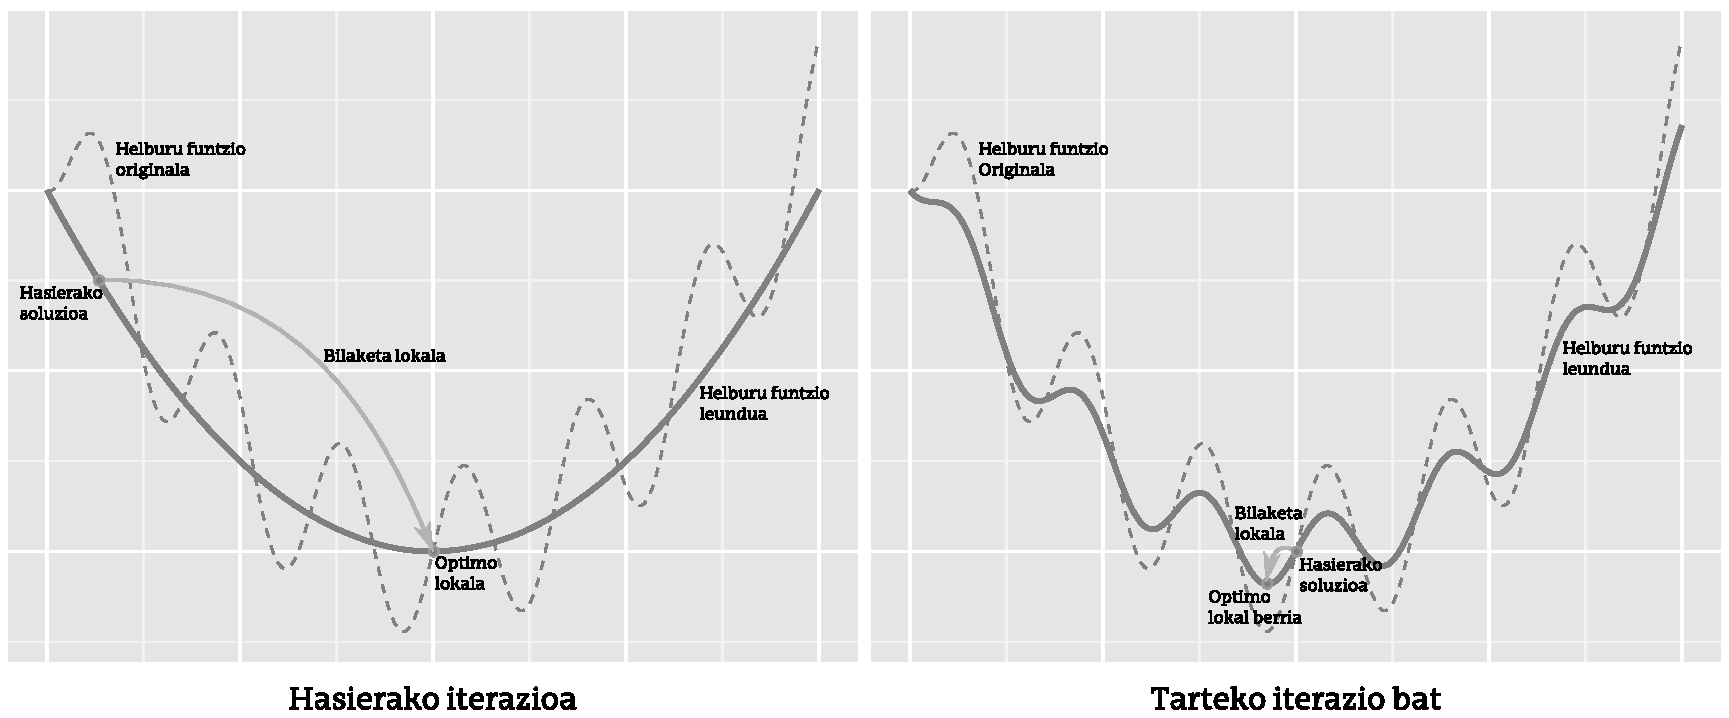
\includegraphics[width=\linewidth]{./Irudiak/smoothing}
\caption{\textit{Smoothing} algoritmoaren funtzionamendua. Iterazio bakoitzean hasierako helburu funtzioa maila bateraino leuntzen da eta bilaketa lokala aplikatzen da.}
\label{fig:smoothing}
\end{figure}

Helburu funtzioa nola leundu problemaren araberakoa erabakia da. Edonola ere, kasu guztietan, algoritmoa inplementatu ahal izateko leuntze-parametro bat definitu beharko dugu. Parametro hau handia denean, helburu funtzioa asko leunduko dugu; parametroa 1 denean, berriz, helburu funtzioa ez da bat ere aldatuko. Hau aintzat hartuz, \ref{alg:smooth} algoritmoan metodoaren sasikodea definituta dago. Ikus dezagun adibide bat.

\begin{ifalgorithm}[t]
\begin{ifpseudo}{Oinarrizko \textit{Smoothing} algoritmoaren sasikodea}
\item \In\ \textit{smoothing ($f$,$\alpha$)} helburu funtzioa eraldatzeko funtzioa
\item \In\ \textit{local\_search($s$,$f$)} bilaketa lokala
\item \In\ \textit{update($\alpha$)} faktorea eguneratzeko funtzioa
\item \In\ $s$ hasierako soluzioa; $\alpha_0$ hasierako faktorea; $f$ helburu funtzioa
\item  $s^* = s$; $\alpha=\alpha_0$
\item \While {$\alpha > 1$} \Do
\item \T{$f^\prime = $\textit{smoothing}($f$;$\alpha$)}
\item \T{$s^* = $\textit{local\_search}($s^*$,$f^\prime$)}
\item \T{$\alpha = $\textit{update}($\alpha$)}
\item \Done
\end{ifpseudo}
\caption{\textit{Smoothing} algoritmoaren sasikodea}\label{alg:smooth}
\end{ifalgorithm}


\begin{tcolorbox}
\begin{ifexample}

TSP-an helburu funtzioa kalkulatzeko distantzien matrizea erabiltzen dugu. Matrize horretan edozein bi hirien arteko distantzia dago jasota. Helburu funtzioa leuntzeko, matrizea hau eralda daiteke, distantzia guztiak batez-besteko distantziara hurbilduz, adibidez. Demagun ondoko matrizea definitzen dugula:

\begin{align}
\renewcommand*{\arraystretch}{1.5}
d_{ij}(\alpha) = \left\{
\begin{array}{ll}
\bar{d} + (d_{ij} - \bar{d})^\alpha &\ \ \mbox{baldin eta } d_{ij}\geq \bar{d}\\
\bar{d} - (\bar{d} - d_{ij})^\alpha &\ \ \mbox{baldin eta } d_{ij} < \bar{d}
\end{array}\right.
\end{align}

\noindent non $\bar{d}$ distantzien batez-bestekoa eta $d_{ij}$ jatorrizko matrizearen elementuak diren. Distantzia matrizea normalizatuta badago -- distantzia guztiak 1 edo txikiagoak badira\footnote{Kontutan hartu behar da, matrizea normalizatuta ere, soluzio optimoa, hau da, balio minimoa duena, ez dela aldatzen.} -- $\alpha$ parametroa oso handia denean distantzia guztiak batez-bestekoari hurbilduko zaizkio, $0\leq (d_{ij} - \bar{d}),(\bar{d} - d_{ij})<1$ baita. Muturreko kasu horretan, soluzioa tribiala da, soluzio guztiak berdinak baitira. 

Iterazioz iterazio $\alpha$ parametroa gutxituko dugu, 1 baliora heldu arte. Goiko ekuazioan ikus daitekeen bezala, $\alpha=1$ denean distantzia matrizea jatorrizkoa da.
\end{ifexample}
\end{tcolorbox}


\bibliographystyle{plain}
\bibliography{references}

\end{document}
